\documentclass[12pt]{article}
\usepackage[margin=1in]{geometry}
\usepackage{setspace}
\doublespacing
\usepackage{graphicx}
\usepackage{booktabs}
\usepackage{amsmath}
\usepackage{amssymb}
\usepackage{caption}
\usepackage{float}
\usepackage{hyperref}
\usepackage[style=apa,backend=biber,natbib=true]{biblatex}
\addbibresource{../references/local_income_taxes.bib}
\usepackage{bm}

\newcommand{\sym}[1]{\textsuperscript{#1}}

\hypersetup{
    colorlinks=true,
    linkcolor=black,
    citecolor=black,
    urlcolor=blue
}

\title{When Do Local Income Taxes Cause Residential Sorting? \\
\large Evidence from Pennsylvania's Piecewise EIT System}
\author{Matthew Hockert\thanks{University of Minnesota. Email: hocke069@umn.edu}}
\date{\today}

\begin{document}

\maketitle

\begin{abstract}

\end{abstract}

\newpage

%==========================================================
\section{Introduction}
\label{sec:intro}
%==========================================================

The Tiebout hypothesis predicts that residents sort across
jurisdictions which offer different fiscal amenities and different costs and residents will 'vote with their feet' and choose specific bundles of amenities for a given amount of taxation, called the Tiebout margin \citep{tiebout1956}. A survey of the literature conducted by \citet{agrawalLessonsStateLocal} highlights the current findings of state and local income taxation and identifies sub-state (county, municipality, school districts) income-tax sorting as one of the field's open questions.
The literature has focused mostly on state tax adjustments on high-earners
\citep{young2016, agrawalRelocationRichMigration2019}. The research shows that
top-income households are generally mobile when rates between states are large, and \citet{agrawal2015gradient} documents sharp discontinuities among commodity-taxes at sub-state borders, but does not estimate the sub-state Tiebout margin for income taxes. The closest existing research comes from
\citet{yangRESPONSIVENESSINCOMELOCAL2017} which  finds small migration effects for county-level income tax adjustments in Indiana.

This paper estimates municipal-level migration effects among workers in Pennsylvania from 2002--2019, by merging local income tax data with the LEHD Origin-Destination
Employment Statistics (LODES), which links each worker's residence to their workplace at annual
frequency and at sub-municipal geography. In Pennsylvania there are roughly $2{,}500$ municipalities and $500$ school districts (SD) that set
their own Earned Income Tax (EIT) rates
\citep{bagchiEffectsIntroducingWithholding2022,agrawalLessonsStateLocal},
producing a deep cross-section of multiple sub-state income-tax opportunities. The EIT offers two additional dimensions of variation that my
empirical design exploits. First, the EIT is set independently by two
overlapping rate-setting jurisdictions (municipalities and school
districts) and a resident's home-side tax bill is the sum of the
municipal resident rate and the school-district rate. This paper's primary
focus is the municipal resident rate while the school district rate enters the empirical
design but is treated as secondary.
Second, the EIT operates using a piecewise maximization rule where each worker's bill is
$T = \max(\tau^{\text{home}}, \tau^{\text{nr,muni}}_{\text{work}})$, where
$\tau^{\text{home}} = \tau^{\text{res,muni}} + \tau^{\text{SD}}$ is the
sum of the municipal resident rate and the school-district resident
rate at the worker's address (the home stack), and $\tau^{\text{nr,muni}}_{\text{work}}$ is the
nonresident rate of the worker's workplace municipality. A statutory home-side rate
change only moves the bill if the home stack is on the binding side
of the max. Act~32 of 2008 (effective 2012) consolidated EIT
collection into county-based Tax Collection Districts and mandated
employer withholding at the higher of the two rates, which made the
max-rule mechanically enforced.
\citet{bagchiEffectsIntroducingWithholding2022} estimates that Act~32 resulted in a $14 \%$ increase in compliance and much higher local revenues. My paper does not analyze compliance but rather estimates
residential-sorting and provides additional analysis pre-post Act~32.

Beyond contributing to the general literature on local tax rate changes and residential sorting  this paper's methodological contribution is utilizing the piecewise structure of the EIT to generate a binding decomposition to test how rate changes that move the tax bill from the non-resident side to resident side and producing a within-design placebo. A statutory rate change moves the worker's bill only when the home stack is on the binding side of the
maximization function, but that same statutory change produces a predicted-null when
the home stack stays below the work-side nonresident rate. Splitting
rate-change events by whether or not they are binding isolates
whose bill actually moves and those whose bill does not. Splitting rate-change events by binding state isolates the rate hikes that actually move the worker's bill and this within-design heterogeneity is what \citet{agrawalLessonsStateLocal} identifies as missing from the existing U.S. local-income-tax literature.
The decomposition is implemented at the municipality-year level in
a continuous stacked difference-in-differences design that uses
never-changed municipalities as the control pool. The
school-district rate enters the design as a co-treatment on the
home-side stack but is not used as a separate unit of analysis.
Section~\ref{sec:theory} formalizes the binding decomposition and
lays out the worker-bill differencing function each cell implies.

The headline causal estimate is the municipality-level Inc-bind
coefficient: at the typical Inc-bind dose of $0.24$ pp cumulative
over five years, the muni-rate change reduces the log count of
workers who both live and work in the municipality by roughly
$13\%$ ($\beta = -0.573$ per pp, $0.24 \times -0.573 = -0.14$ log
points), with clean pre-trends (joint Wald $p = 0.33$) and a null
Inc-nobind within-design placebo. The per-pp coefficient should be
read as the regression slope, not a typical-event headline: a $1$
pp shock is two to three standard deviations above the median
realized dose. The Inc-bind cohort is also small (24
municipalities, mostly Home Rule boroughs in eastern PA), so the
estimate is a local treatment effect for binding rate-raisers
rather than a state-average elasticity.

The remainder of the paper is organized as follows.
Section~\ref{sec:background} describes the institutional setting and
Act~32. Section~\ref{sec:theory} introduces the six-cell binding
decomposition. Section~\ref{sec:data} describes the downloading and merging of the multiple data sources: LODES, the DCED rate
panel, and the municipal and school-district controls.
Section~\ref{sec:strategy} explains the continuous stacked
difference-in-differences design at the municipality level.
Section~\ref{sec:results} reports the pooled benchmark and the
municipality-level causal headline.
Section~\ref{sec:robustness} reports robustness diagnostics, and
Section~\ref{sec:discussion} concludes.

%==========================================================
\section{Institutional Background}
\label{sec:background}
%==========================================================

Pennsylvania has a deep cross-section of jurisdictions setting
their own income tax rate: approximately 2{,}500 municipalities and 500 school
districts each levy a separate Earned Income Tax on essentially
all earned income earned in or by Pennsylvania residents
\citep{bagchiEffectsIntroducingWithholding2022,agrawalLessonsStateLocal}.
Unlike property taxes, which are paid by owners and capitalized into
home values, the EIT falls directly on workers and varies across
municipal boundaries, creating
sharp spatial discontinuities in tax burden that can influence where
workers choose to live and work.

\subsection{Pennsylvania Earned Income Tax}
\label{subsec:pennsylvania}

Pennsylvania's EIT is mandatory for all municipalities under the
Local Tax Enabling Act of 1965 \citep[Act 511;][]{paAct511_1965}.
It applies to all earned income with no minimum threshold. The standard combined cap is 1\%, typically split as
0.5\% municipal and 0.5\% school district. Home Rule municipalities
may exceed this cap \citep{paHomeRule}, and Philadelphia operates
separately under the Sterling Act of 1932
\citep{paSterlingAct_1932} at approximately 3.9\%. EIT is a valuable revenue funder for local governments next to property-taxes. However, quantifying the effect of property tax millage on sorting would
require a 2002--2019 municipality-level millage panel that is not currently
available from DCED, and I leave the comparison to property-tax
sorting as a separate exercise. Across 2002--2019, the panel contains
210 municipality resident-rate increases, 119 municipality decreases, 611
school-district increases, and 52 school-district decreases; the
binding breakdown of these events is in
Table~\ref{tab:cell_counts_summary}.

Each Pennsylvania municipality has three EIT rates relevant to a
worker:
%
the municipality resident rate $\tau^{\text{res,muni}}$ levied on residents of the municipality, the municipality nonresident rate $\tau^{\text{nr,muni}}$ levied on workers employed in the municipality who live elsewhere, and the school-district rate $\tau^{\text{SD}}$ levied on residents only (school districts cannot tax nonresidents).
%
Each address is associated with a six-digit Political Subdivision (PSD)
code identifying its (municipality, school district) pair. Workers report this
code on the Residency Certification Form, and employers use it to
determine withholding obligations.

Under Act 32 (effective January 1, 2012), a worker's total EIT bill
is determined by the maximum of the home-side rate stack and the
work-location nonresident rate, and the bill is split piecewise
between home and work jurisdictions:
%
\begin{equation}
\bigl(\tau^{\text{home}},\ \tau^{\text{work}}\bigr) =
\begin{cases}
\bigl(\tau^{\text{res,muni}}_j + \tau^{\text{SD}}_j - \tau^{\text{nr,muni}}_i,\ \tau^{\text{nr,muni}}_i\bigr)
   & \text{if } \tau^{\text{res,muni}}_j + \tau^{\text{SD}}_j > \tau^{\text{nr,muni}}_i \\[4pt]
\bigl(0,\ \tau^{\text{nr,muni}}_i\bigr)
   & \text{if } \tau^{\text{res,muni}}_j + \tau^{\text{SD}}_j \leq \tau^{\text{nr,muni}}_i
\end{cases}
\label{eq:piecewise}
\end{equation}
%
where $j$ is the worker's home municipality and $i$ is the work municipality. The
work jurisdiction always collects its full nonresident rate first, then
the home municipality and school district split whatever portion of the
worker's bill is left over after the work claim. If the work nonresident
rate exceeds the home stack, the home jurisdictions get nothing. The
worker's total bill is the higher of the two stacks:
%
\begin{equation}
\text{Bill}_{ji} = \max\!\bigl(\tau^{\text{res,muni}}_j + \tau^{\text{SD}}_j,\ \tau^{\text{nr,muni}}_i\bigr).
\label{eq:bill}
\end{equation}

Equation~(\ref{eq:piecewise}) implies which margin a worker can use to
respond to a rate increase. When the home stack binds
($\tau^{\text{home}}_j > \tau^{\text{nr,muni}}_i$), the worker can lower
the bill only by moving home to a lower-rate municipality or school district.
When the work nonresident rate binds, the worker can lower the bill
only by changing jobs to a lower-nonres-rate work location, while moving homes
without changing jobs has no effect. For workers who live and work in
the same municipality, only the home stack applies(
$\tau^{\text{res,muni}}_i + \tau^{\text{SD}}_i$).

A worker who lives in municipality $j$ and moves to a lower-rate municipality $j'$
while keeping the same job at $i$ saves at least the SD rate at $j$:
the new bill is $\max(\tau^{\text{home}}_{j'}, \tau^{\text{nr}}_i)$,
which is at most the old bill $\tau^{\text{home}}_j$ minus
$\tau^{\text{SD}}_j$. The empirical design follows this logic directly: both the treatment
$\Delta\tau^{\text{muni}}$ and the binding classification are
built from the worker's home stack. The regressions therefore measure
sorting in response to the same tax a mover would actually face.

Philadelphia is the one exception to the Act 32 framework. It operates under
the Sterling Act of 1932 where Philadelphia residents pay the city resident
rate regardless of work location with no offset and Philadelphia
nonresidents pay the city nonresident rate, with no residual flowing
to home jurisdictions in other Pennsylvania municipalities. My main estimates
retain Philadelphia in the sample for completeness and the results are robust
to dropping it.

Act 32 transformed the system by consolidating collection into
approximately 67 county-based Tax Collection Districts (TCDs), each with a single appointed collector.
The law mandated standardized employer withholding at the higher of
the employee's resident and work rate. This had two consequences.
First, it made the EIT mechanically binding where the rate changes now
appear in every worker's paycheck through employer withholding,
regardless of whether the worker resides in the taxing municipality.
Second, it eliminated the possibility of avoidance
of the work-location nonresident claim through weak enforcement.
After Act 32, a worker could no longer effectively duck the
nonresident portion owed to the work municipality.

However, Act 32 did not eliminate all tax savings from
residential relocation. The piecewise rule in
Equation~(\ref{eq:piecewise}) continues to imply that a worker whose
original home stack binds can reduce the bill by moving to a
sufficiently lower-stack home jurisdiction where the new bill is
$\max(\tau^{\text{home}}_{j'}, \tau^{\text{nr}}_i)$, which falls
below the old home stack $\tau^{\text{home}}_j$ whenever
$\tau^{\text{home}}_{j'} < \tau^{\text{home}}_j$ and the original
home stack was the binding side. Act 32 thus changed enforcement
and made the max-rule mechanically binding through withholding; it
did not eliminate the residential-relocation margin that the
mechanism in this paper exploits.
\citet{bagchiEffectsIntroducingWithholding2022} documents the
quantitative consequences of Act 32 directly: consolidated employer
withholding increased PA EIT compliance, raised reported earned
income in the rate-raising municipality, and shifted the de facto incidence
toward workers. The present paper complements that work by isolating
the residential-sorting response to the same withholding-enforcement
regime, exploiting the cross-sectional variation in whether a given
rate change actually moves the worker's bill (the binding
decomposition); the pre/post-Act-32 split in
Section~\ref{sec:robustness} shows the binding-cell sorting
response strengthens (the effect existed prior to Act 32) after Act 32, complementing the
compliance-response finding.

Figure~\ref{fig:act32_cdf} documents the institutional break at
Act 32. Before 2012, fewer than 60\% of PA municipalities reported a
nonresident rate to DCED; after 2012, when consolidated withholding
made the max-rule mechanically binding, coverage rises sharply.
This is the pre-/post-Act-32 enforcement break used in the
heterogeneity test of Section~\ref{subsec:rob-act32}.

\begin{figure}[H]
    \centering
    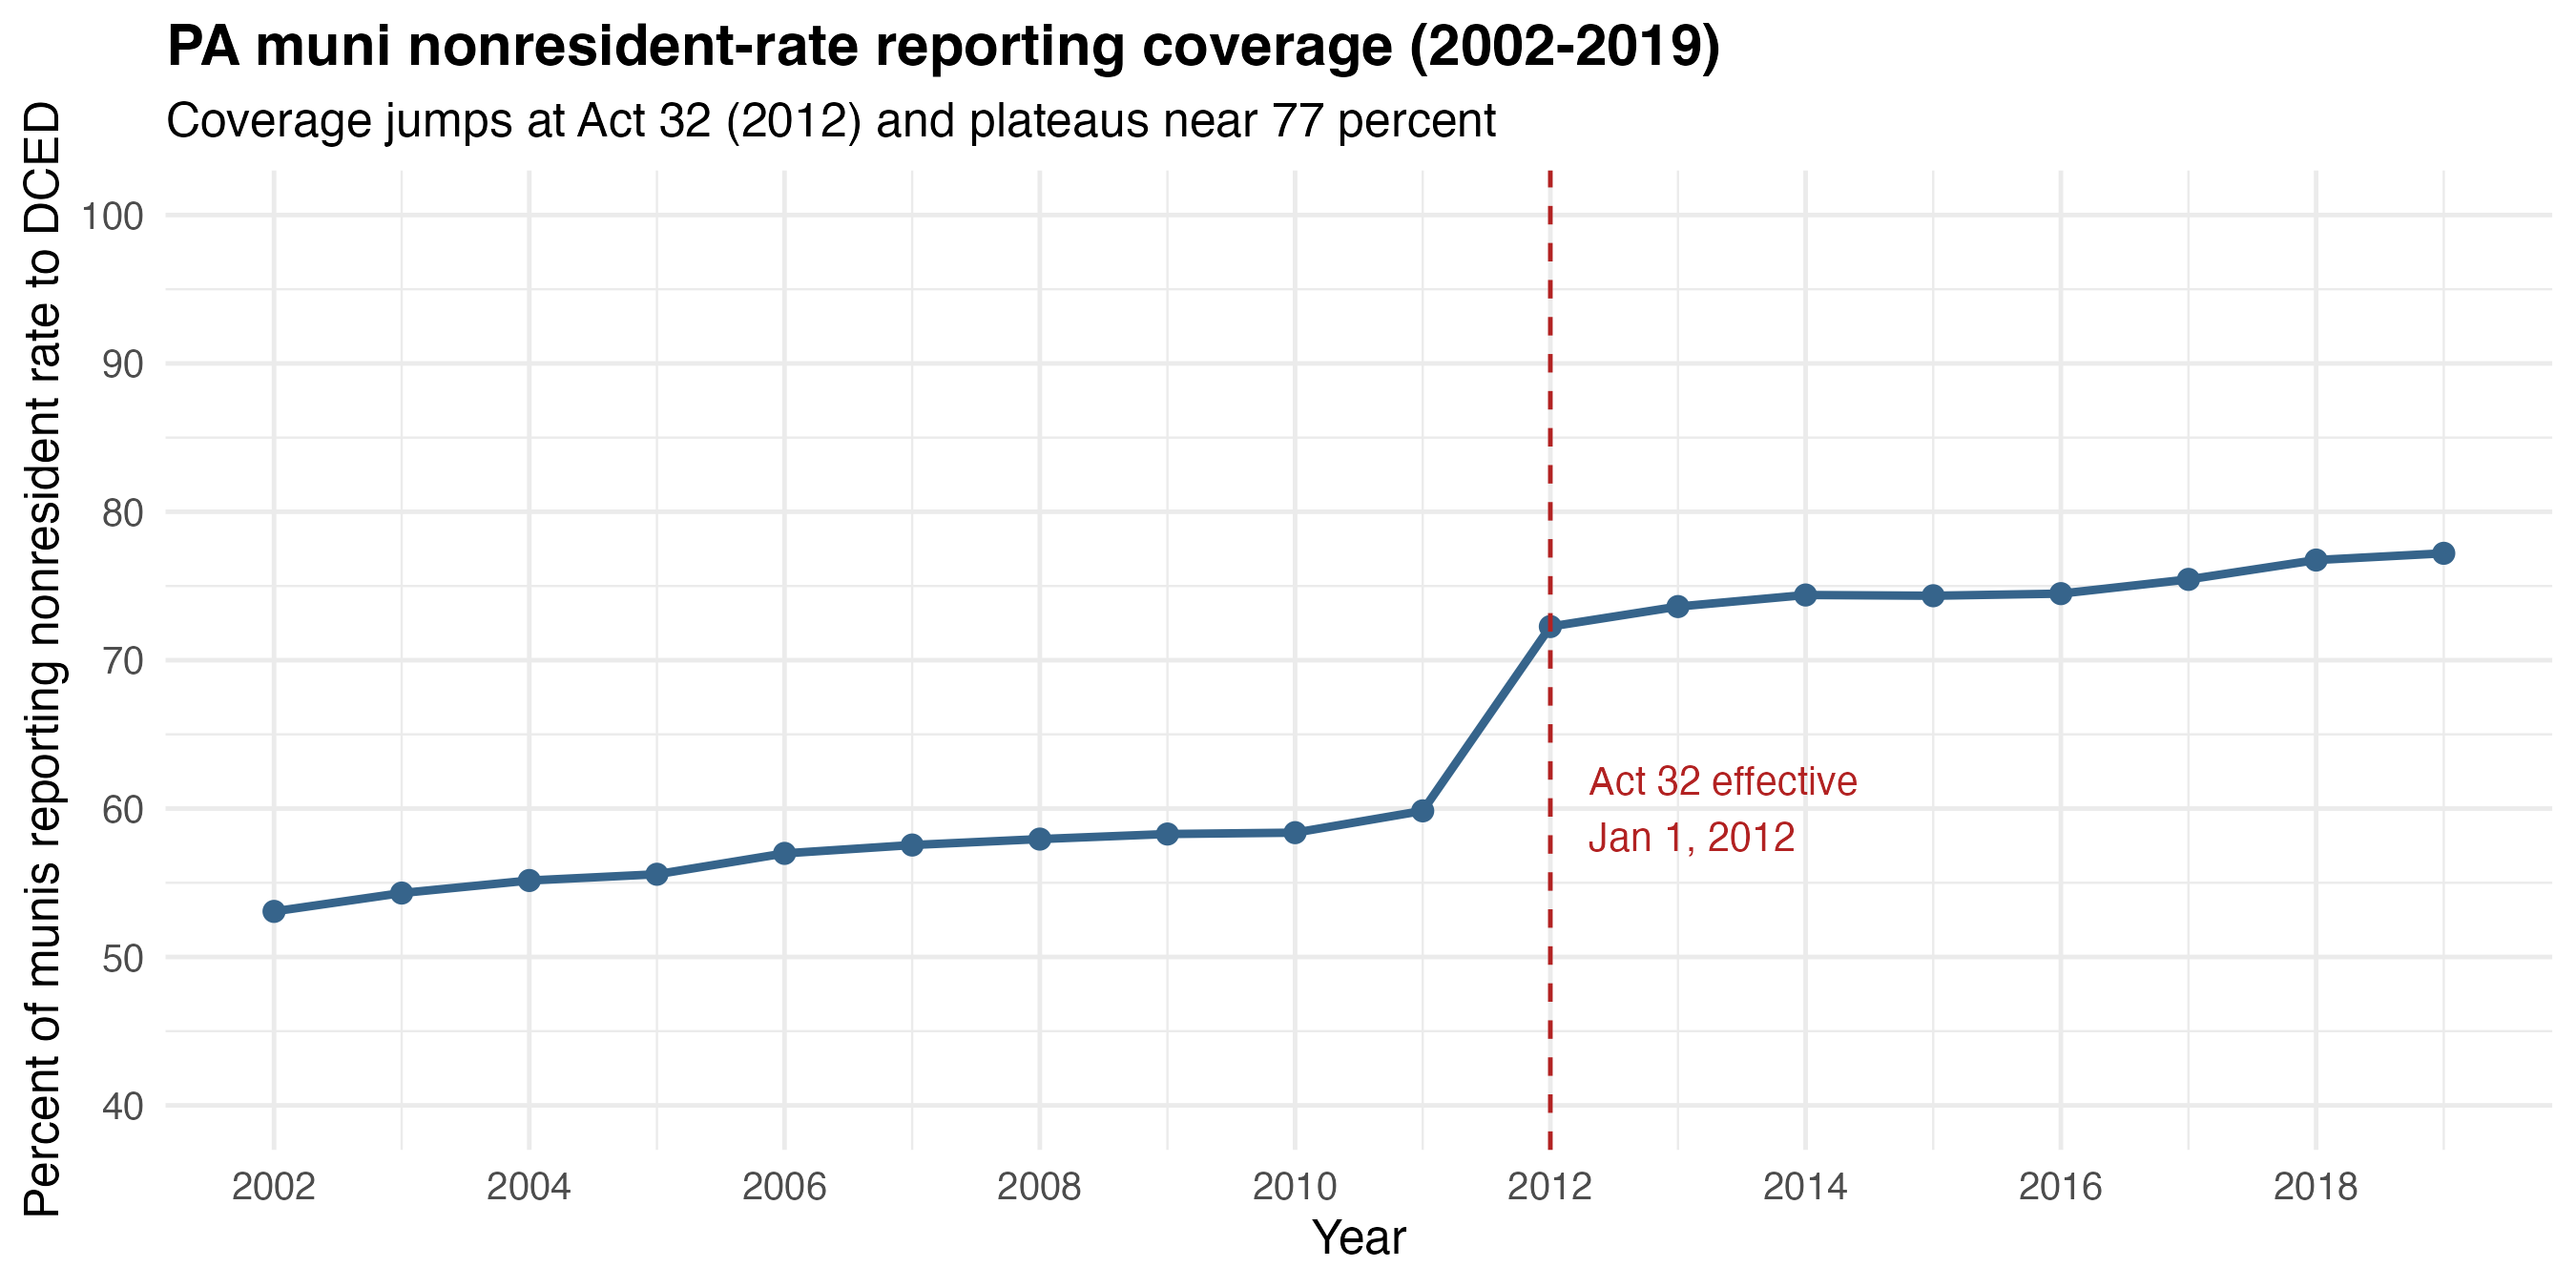
\includegraphics[width=0.85\textwidth]{../figures/nonres_coverage.png}
    \caption{Share of PA municipalities reporting a nonresident
    rate to DCED, by year. The break at 2012 reflects the Act 32
    requirement that employers withhold at the higher of the home
    resident and work nonresident rates.}
    \label{fig:act32_cdf}
\end{figure}

School districts in Pennsylvania also levy an EIT under Act 511
\citep{paAct511_1965}, typically at 0.5\% (the other half of the
standard 1\% cap). Act 1 of 2006 \citep{paAct1_2006} (the Taxpayer
Relief Act) additionally authorized
school districts to exceed the 0.5\% cap specifically to fund
property tax relief. This generated a wave of school district
rate increases in 2006--2011, creating rate variation that is independent of municipal fiscal decisions. I find that the correlation between the municipal and school-district resident rates is only weakly negative of $-0.12$ indicating the two taxing jurisdictions move on relatively separate schedules. Since every census tract sits in both a municipality
and a school district, workers face two overlapping EIT rates
that can change independently, providing a natural decomposition
of the residential sorting response into municipal and school
district components.

%==========================================================
\section{Conceptual Framework: Binding Decomposition}
\label{sec:theory}
%==========================================================

The piecewise tax allocation in Equation~(\ref{eq:piecewise}) is the causal
identification backbone of my empirical design. A worker's bill is
$T = \max(\tau^{\text{home}}, \tau^{\text{nr,muni}}_{\text{work}})$. A rate change
only moves the bill when its side of the max binds. The
implied change in the worker's bill from a single rate event is
\[
  \Delta T \;=\; \max(\tau^{\text{home}}_{\text{post}}, \tau^{\text{nr}})
              - \max(\tau^{\text{home}}_{\text{pre}},  \tau^{\text{nr}}),
\]
which depends jointly on the direction of the rate change and on
which side of the max is binding pre- and post-event. This tax difference from pre and post rate changes can
produce a strong behavioral response, a moderate response, or no
response at all depending on the binding transition.

\subsection{Six Cells per Rate-Setter}
\label{subsec:cells}

Two definitions structure the decomposition. First, the piecewise
rule $T = \max(\tau^{\text{home}}, \tau^{\text{nr,muni}}_{\text{work}})$ has two
sides: the home side
$\tau^{\text{home}} = \tau^{\text{res,muni}} + \tau^{\text{SD}}$,
set at the worker's residence, and the work side
$\tau^{\text{nr,muni}}_{\text{work}}$, the nonresident rate set by the worker's workplace municipality.
Whichever side is larger is the binding side and determines
the bill. Second, three rate-setters adjust statutory rates
independently across municipality-years: the municipality resident
rate $\tau^{\text{res,muni}}$, the school-district rate
$\tau^{\text{SD}}$, and the municipality nonresident rate
$\tau^{\text{nr,muni}}$. The decomposition is built one rate-setter
at a time.

For each rate-setter $\tau$, a cell classifies a municipality
by (i)~the direction of its first rate event in $\tau$ (Increase or
Decrease) and (ii)~the binding transition of its home stack
across that event: stayed-binding, flipped, or stayed-non-binding.
The cross gives six cells plus a seventh never-changed control pool,
of which only the three Increase cells and the NC control are used in
this paper (Table~\ref{tab:cells}). Each municipality therefore carries three
cell labels (one for each of $\tau^{\text{res,muni}}$,
$\tau^{\text{SD}}$, and $\tau^{\text{nr,muni}}$) and the binding
state for each is determined by where its home stack sits relative
to its nonresident rate at the time of that event.

\begin{table}[H]
\centering
\small
\begin{tabular}{lcccl}
\toprule
Cell & Direction & Pre-binding? & Post-binding? & Bill effect \\
\midrule
Inc-bind         & $\uparrow$  & yes & yes & rises by full $\Delta\tau$ \\
Inc-becomes      & $\uparrow$  & no  & yes & rises by part of $\Delta\tau$ \\
Inc-nobind       & $\uparrow$  & no  & no  & no change (placebo) \\
NC               & none & --- & --- & control pool \\
\bottomrule
\end{tabular}
\caption{Binding cells per rate-setter on the increase side. For Inc-becomes the bill rises only by the portion of $\Delta\tau$ above the nonresident rate. Three mirror decrease cells exist by construction but are not estimated in this paper because the decrease cohort is too thin to support causal inference ($4$ Dec-bind, $3$ Dec-becomes-non, $11$ Dec-nobind) and the realized-dose pre-trend rejects parallel trends on every Dec outcome.}
\label{tab:cells}
\end{table}

The cell labels describe the \emph{state of the home stack at the
rate event}, not which rate-setter is responsible for that state.
The home stack $\tau^{\text{home}} = \tau^{\text{res,muni}} + \tau^{\text{SD}}$ is
additive in its two home-side components; either component can put
the stack above or below the nonresident floor. The muni-side cell
label asks: at the year of the municipality's first resident-rate
event, was the home stack above the nonresident rate pre- and
post-event? The SD-side cell label asks the same question
evaluated at the year of the SD's first rate event. A municipality
therefore carries two independent cell labels, one for each
rate-setter, and the two are not mutually exclusive: a muni
classified as Inc-bind on the muni side may be Inc-becomes on the
SD side (or any other combination). The interaction terms in the
estimating equation (Section~\ref{sec:strategy}) separate the
per-pp effect of a muni-rate change from the per-pp effect of an
SD-rate change, each conditional on its own cell label.

What the labels imply for an individual worker depends on where
that worker is employed. Under Act~32 the employer withholds at
$\max(\tau^{\text{home}}, \tau^{\text{nr,muni}}_{\text{work}})$, where
$\tau^{\text{nr,muni}}_{\text{work}}$ is the nonresident rate of the
\emph{worker's workplace} \citep{paAct32_2008, bagchiEffectsIntroducingWithholding2022}. For a worker who lives \emph{and} works in
municipality $X$ the workplace nonresident rate is exactly $X$'s
own $\tau^{\text{nr,muni}}_X$, which is the comparison floor the cell
classification uses; the bill-effect column of
Table~\ref{tab:cells} is therefore institutionally exact for this
sub-population. For a resident of $X$ who works in a different
municipality $Y$, the relevant floor is $\tau^{\text{nr,muni}}_Y$,
which the LODES origin--destination data does not let us recover at
the worker level; here the muni-side cell label using $X$'s own
nonresident rate is an aggregate proxy that is reasonable on
average across Pennsylvania's local commute shed but not verifiable
individually. This distinction motivates the outcome ordering in
Section~\ref{sec:results}: the count of workers who live and work
in their own municipality, $\log(\text{live-and-work})$, is the
cleanest binding-rule test because the classification matches each
worker's actual workplace; counts that mix the live-and-work and
out-commuter populations
($\log(\text{employed residents})$, share live-in) inherit the
out-commuter proxy uncertainty; and $\log(\text{in-commuters})$
does not test the muni resident-rate binding rule at all because
in-commuters' bills do not depend on the resident rate of the
municipality where they work.

The fundamental testable prediction is an
ordered ranking of cell magnitudes where Inc-bind effects exceed
Inc-becomes effects, which in turn exceed Inc-nobind effects, with
the last close to zero and serving as the
within-design placebo. A tax salience argument would state that workers in the Inc-becomes cell
experience a discrete switch from paying zero home-side tax to
paying a positive amount, which should trigger a large behavioral response. The
central empirical comparison of the paper is between Inc-bind and
Inc-nobind where if statutory rates matter mechanically through tax
liability, the residential response should appear in Inc-bind and
not in Inc-nobind. If Inc-nobind moves, the mechanism
interpretation fails and the response is something other than the
binding rule because Inc-nobind events do not change the worker's
bill. This makes the design self-falsifying in a way that a
conventional pooled-Increase specification is not. In the pooled
specification, every increase is a treated event, while here the
institutional rule predicts that only a subset of statutory
increases should generate a response.

%==========================================================
\section{Data}
\label{sec:data}
%==========================================================

\subsection{Data Sources}
\label{subsec:sources}
\label{subsec:sample}
\label{subsec:pipeline}

The analysis merges the LEHD  residence--workplace dataset and the  Pennsylvania EIT rate records to create a panel of rate changes and workforce data over space and time. The two datasets do not share common identifiers, and was bridged using TIGER~2020 block geometry, which
nests blocks within county subdivision code(cousubs). A
municipality-name crosswalk maps each DCED municipality ID to its
corresponding COUSUBFP code, matching $2{,}496$ of $2{,}505$ PA municipalities
($99.6\%$). The remaining $9$ are small boroughs that have either dissolved or
merged during 2002--2019 and are dropped from the analysis.

The residence--workplace data come from LEHD LODES Version~8,
2002--2019 \citep{lehdLODES}. The Census Bureau applies
synthetic noise infusion at the block level to protect respondent
confidentiality and is calibrated so that aggregation to tract and larger
geographies approximates ground truth
\citep{grahamDESIGNCOMPARISONLODES}. The sample period of 2002--2019
reflects LODES coverage beginning in 2002 and
2020--2023 to not include disruptions in the data resulting from the COVID Pandemic.

Municipal and school-district EIT rates come from the Pennsylvania
Department of Community and Economic Development (DCED) MunStats
portal \citep{padcedMunStats}, scraped annually. In some DCED reports, the flat-dollar Local Services Tax is filled in the same field
as the EIT in some years, so rates above $5\%$ are treated as
data-entry errors and dropped except for Home Rule cities and Philadelphia.

Municipal fiscal controls come from the PA DCED Statewide Municipal
Annual Financial Report database \citep{padcedAFR}. School-district
fiscal controls come from the Census Annual Survey of School System
Finances (F-33) \citep{censusF33}; the NCES \texttt{LEAID}-to-DCED
SD ID crosswalk covers all $500$ school districts. All fiscal
controls are share-based and time-varying. Municipality regressions
use six DCED AFR shares: three expenditure shares
(police-services, streets, debt-service) and three revenue shares
(EIT-revenue, real-estate-tax, intergovernmental-revenue).
LODES blocks are aggregated to muni for analysis.

The municipality--SD assignment uses the modal SD ID per muni in
the DCED rate panel ($97.6\%$ of municipalities are single-SD), so
each muni-year carries a single $\tau^{\text{SD}}$ co-treatment.
Municipality regressions
further impose a
minimum employment threshold of $50$ total jobs, which protects the
share-based outcomes from mechanical noise (a single worker moving
changes a share by $1/N$, so at $N=10$ a one-worker move dominates
the per-pp coefficient) and matches the LODES synthetic-noise
calibration that is validated at tract scale and above
\citep{grahamDESIGNCOMPARISONLODES}. The threshold drops $185$ of
$2{,}559$ municipalities ($7.2\%$), almost all sparsely populated
NC-pool townships; the treated cohort is essentially unaffected.
Sensitivity analysis in Section~\ref{sec:robustness} confirms the
Inc-bind coefficient is stable across thresholds from $10$ to $500$.

\subsection{Descriptive Statistics}
\label{subsec:descriptive}

This section presents the summary statistics at the municipality
level. The primary outcome variables are resident-worker counts,
workplace counts, in-commuter flows, and the live-and-work share.
Fiscal outcomes used as control variables (log EIT revenue, log
total tax revenue, log total revenue, log police expenditure) are
reported in Appendix~\ref{app:robustness}.

Table~\ref{tab:summary_muni} summarizes the estimation panel.

% (block summary removed; muni is the only estimating unit)
% \begin{table}[H]
  \centering
  \caption{Block-year summary statistics (2002--2019)}
  \label{tab:summary_block}
  \small
  \resizebox{\textwidth}{!}{
  \begin{tabular}{lrrrrrrrr}
    \toprule
    Variable & N & Mean & SD & p25 & p50 & p75 & Min & Max \\
    \midrule
    Home count (workers living) & 5,030,958 & 18.822 & 31.677 & 4.000 & 10.000 & 22.000 & 0.000 & 1572.000 \\
    $\log$ home count & 4,795,213 & 2.293 & 1.198 & 1.386 & 2.398 & 3.135 & 0.000 & 7.360 \\
    Work count (jobs in block) & 5,030,958 & 18.826 & 138.957 & 0.000 & 0.000 & 4.000 & 0.000 & 20945.000 \\
    $\log$ work count & 1,894,432 & 2.256 & 1.663 & 1.099 & 2.079 & 3.367 & 0.000 & 9.950 \\
    Share live-and-work in muni & 4,795,213 & 0.154 & 0.222 & 0.000 & 0.067 & 0.203 & 0.000 & 1.000 \\
    Share work outside muni & 4,795,213 & 0.846 & 0.222 & 0.797 & 0.933 & 1.000 & 0.000 & 1.000 \\
    Resident rate $\tau^{M}$ (\%) & 4,782,928 & 0.762 & 0.799 & 0.500 & 0.500 & 0.500 & 0.000 & 4.331 \\
    SD rate $\tau^{SD}$ (\%) & 4,782,928 & 0.607 & 0.376 & 0.500 & 0.500 & 0.500 & 0.000 & 2.050 \\
    Nonresident rate $\tau^{nr,M}$ (\%) & 4,181,214 & 1.063 & 0.657 & 1.000 & 1.000 & 1.000 & 0.000 & 3.820 \\
    Blocks per muni & 2,561 & 120.922 & 384.585 & 41.000 & 73.000 & 132.000 & 1.000 & 16550.000 \\
    \bottomrule
  \end{tabular}
  }
  \vspace{0.3em}
  \begin{minipage}{0.95\textwidth}
    \footnotesize \textit{Notes:} Block-year level; one observation per (census block, year). Panel covers 309,680 blocks in 2,561 municipalities.
  \end{minipage}
\end{table}


\begin{table}[H]
  \centering
  \caption{Muni-year summary statistics (2002--2019)}
  \label{tab:summary_muni}
  \small
  \resizebox{\textwidth}{!}{
  \begin{tabular}{lrrrrr}
    \toprule
    Variable & N & Mean & SD & Min & Max \\
    \midrule
    Resident rate $\tau^{M}$ (\%) & 43,374 & 0.525 & 0.163 & 0.000 & 4.331 \\
    Nonresident rate $\tau^{nr,M}$ (\%) & 34,080 & 0.883 & 0.237 & 0.000 & 3.820 \\
    SD rate $\tau^{SD}$ (\%) & 43,374 & 0.622 & 0.289 & 0.000 & 2.050 \\
    Home stack $\tau^{M}+\tau^{SD}$ (\%) & 43,374 & 1.147 & 0.316 & 0.000 & 4.331 \\
    $\log$ live-and-work & 40,748 & 3.638 & 2.011 & 0.000 & 12.877 \\
    $\log$ total jobs & 45,291 & 5.819 & 2.006 & 0.000 & 13.353 \\
    Share live-and-work in muni & 45,291 & 0.095 & 0.081 & 0.000 & 1.000 \\
    \bottomrule
  \end{tabular}
  }
  \vspace{0.3em}
  \begin{minipage}{0.95\textwidth}
    \footnotesize \textit{Notes:} Muni-year level; one observation per (municipality, year). Rates in percentage points. $\tau^{nr,M}$ has reporting gaps before Act 32; the $N$ for that row is smaller than the full panel.
  \end{minipage}
\end{table}


Table \ref{tab:summary_muni} presents the municipality level summary statistics. Table \ref{tab:summary_muni} shows that there are roughly $43{,}374$ muni-year observations, and the resident rate is tightly clustered
near the Act~511 default at $\bar{\tau}^{M}=0.53\%$ and a standard deviation of $0.16$pp. There is a long right tail indicated by the max rate of $4.33\%$ concentrated in Philadelphia and
a handful of Home-Rule and Act~47 distressed cities. The
nonresident rate has $34{,}080$ observation, about $9{,}300$ fewer
observations than the resident rate, due to DCED's lack of coverage for the nonresident-rate field being incomplete before Act~32 mandated
reporting. The SD rate has nearly twice the
muni-rate dispersion (SD $0.29$pp vs.\ $0.16$pp) and maxes at $2.05\%$, potentially making the school-district
rate-setter a larger statistical lever. The home stack averages
$1.15\%$, above the $1\%$ Act~511 cap, because Act~1 SD increases
and Home-Rule muni rates push the upper level past the ceiling.
Outcome variables show that total jobs span $1$ to
$629{,}698$ with an SD of $13{,}032$ on a mean of $2{,}077$, indicating why the regressions use logs. And only $9.5\%$ of muni jobs are
held by residents of the same muni showing that residential sorting operates
on a thin within-muni margin.



% \begin{table}[H]
  \centering
  \caption{School-district-year summary statistics (2002--2019)}
  \label{tab:summary_sd}
  \small
  \resizebox{\textwidth}{!}{
  \begin{tabular}{lrrrrrrrr}
    \toprule
    Variable & N & Mean & SD & p25 & p50 & p75 & Min & Max \\
    \midrule
    SD rate $\tau^{SD}$ (\%) & 49,226 & 0.610 & 0.278 & 0.500 & 0.500 & 0.500 & 0.000 & 2.050 \\
    Resident rate $\tau^{M}$ (\%) (muni-year) & 49,226 & 0.523 & 0.162 & 0.500 & 0.500 & 0.500 & 0.000 & 4.564 \\
    Nonres rate $\tau^{nr,M}$ (\%) (muni-year) & 38,536 & 0.881 & 0.237 & 1.000 & 1.000 & 1.000 & 0.000 & 3.967 \\
    share\_state\_rev\_sd & 9,278 & 0.416 & 0.166 & 0.279 & 0.414 & 0.555 & 0.000 & 0.821 \\
    share\_local\_rev\_sd & 9,278 & 0.536 & 0.186 & 0.376 & 0.536 & 0.691 & 0.103 & 1.000 \\
    share\_federal\_rev\_sd & 9,278 & 0.048 & 0.033 & 0.024 & 0.040 & 0.062 & 0.000 & 0.247 \\
    share\_property\_tax\_sd & 9,278 & 0.420 & 0.176 & 0.270 & 0.407 & 0.562 & 0.000 & 0.853 \\
    share\_instructional\_sd & 9,278 & 0.522 & 0.070 & 0.492 & 0.536 & 0.567 & 0.000 & 1.000 \\
    share\_support\_sd & 9,278 & 0.279 & 0.039 & 0.259 & 0.284 & 0.305 & 0.000 & 0.438 \\
    \bottomrule
  \end{tabular}
  }
  \vspace{0.3em}
  \begin{minipage}{0.95\textwidth}
    \footnotesize \textit{Notes:} SD-year level. F-33 share controls are constructed from Census F-33 revenue/expenditure totals.
  \end{minipage}
\end{table}
  % (SD summary table removed; see paper scope)

\begin{table}[H]
  \centering
  \caption{Cell counts: muni resident-rate side, 2002--2019}
  \label{tab:cell_counts_summary}
  \small
  \begin{tabular}{lrrrr}
    \toprule
    Cell & Munis & Muni-years & Mean dose (pp) & Extreme dose (pp) \\
    \midrule
    Never-changers & 1,730 & 31,132 & 0.000 & 0.000 \\
    Inc-bind & 24 & 432 & 0.168 & 0.850 \\
    Inc-becomes & 43 & 774 & 0.246 & 1.250 \\
    Inc-nobind & 20 & 360 & 0.294 & 0.650 \\
    Dec-bind & 4 & 72 & -0.138 & -0.500 \\
    Dec-becomes-non & 3 & 54 & -0.278 & -0.500 \\
    Dec-nobind & 11 & 198 & -0.380 & -1.000 \\
    \bottomrule
  \end{tabular}
  \vspace{0.3em}
  \begin{minipage}{0.95\textwidth}
    \footnotesize \textit{Notes:} Cells classify each muni's first resident-rate event by direction (Inc/Dec) and the binding-state transition relative to the muni's nonresident rate. NC is the never-changed control pool. Dose is the cumulative $\Delta\tau$ within the 5-year event window. The Extreme dose column reports the max cumulative dose for Inc cells and the min (most negative) cumulative dose for Dec cells, since cell assignment is determined by the first event but subsequent reversals can pull the signed cumulative path back across zero.
  \end{minipage}
\end{table}


Table~\ref{tab:cell_counts_summary} reports the cell
assignments on the muni resident-rate side. Of roughly $2{,}500$
municipalities, $1{,}793$ never change their resident rate and form
the NC control pool; only $194$ are assigned to any treated cell. The three
increase cells split as $24$ Inc-bind, $39$ Inc-becomes, and $14$ Inc-nobind (Table~\ref{tab:cell_counts_summary}). Inc-becomes shows a larger average
dose than Inc-bind, indicating that crossing the binding threshold typically
requires a bigger statutory move than slowly inching up an already-binding
rate. The decrease cells are thin ($4$ Dec-bind, $3$
Dec-becomes-non, and $11$ Dec-nobind). Because of this the decreasing only municipalities generally are not reliable estimates in the results section.

Figure~\ref{fig:rate_changes_by_year} reports the timing of
municipal resident-rate changes across the panel. Increases outnumber
decreases nearly two-to-one overall ($210$ increases vs.~$119$
decreases over 2002--2019), and the gap does not seem to widen after Act~32
took effect in 2012 but the majority of the post-2012 rate-change events
are increases.

\begin{figure}[H]
    \centering
    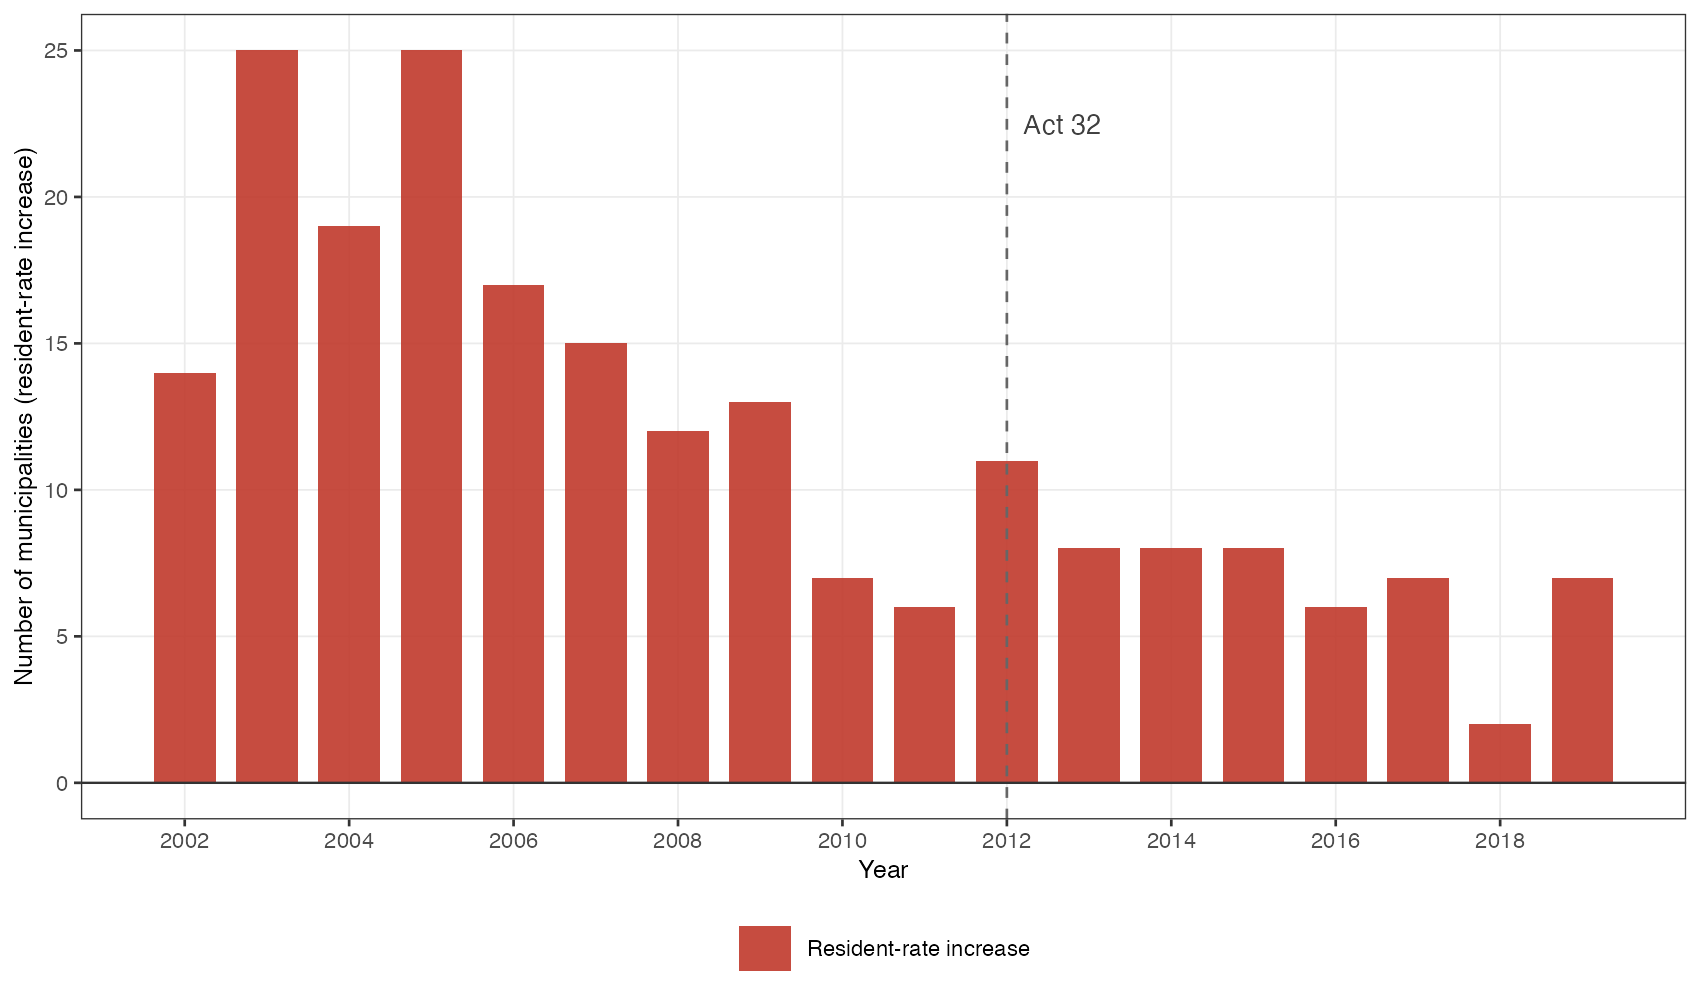
\includegraphics[width=0.95\textwidth]{../figures/rate_changes_by_year.png}
    \caption{Number of PA municipalities changing their resident
    rate, by year. Increases shown above zero; decreases shown below.
    Dashed line: 2012, when Act 32 consolidated withholding.}
    \label{fig:rate_changes_by_year}
\end{figure}

Lastly, figure~\ref{fig:pa_map} shows the spatial distribution of the rate changers in my sample. Most rate changers occur along the east coast, but some are also scattered within the interior of the state. This spatial distribution highlights the value of future work to understand the effects when two neighboring municipalities raise or lower rates across time, which is left for future research. 

% --- Treatment Geography Map ---
\begin{figure}[H]
    \centering
    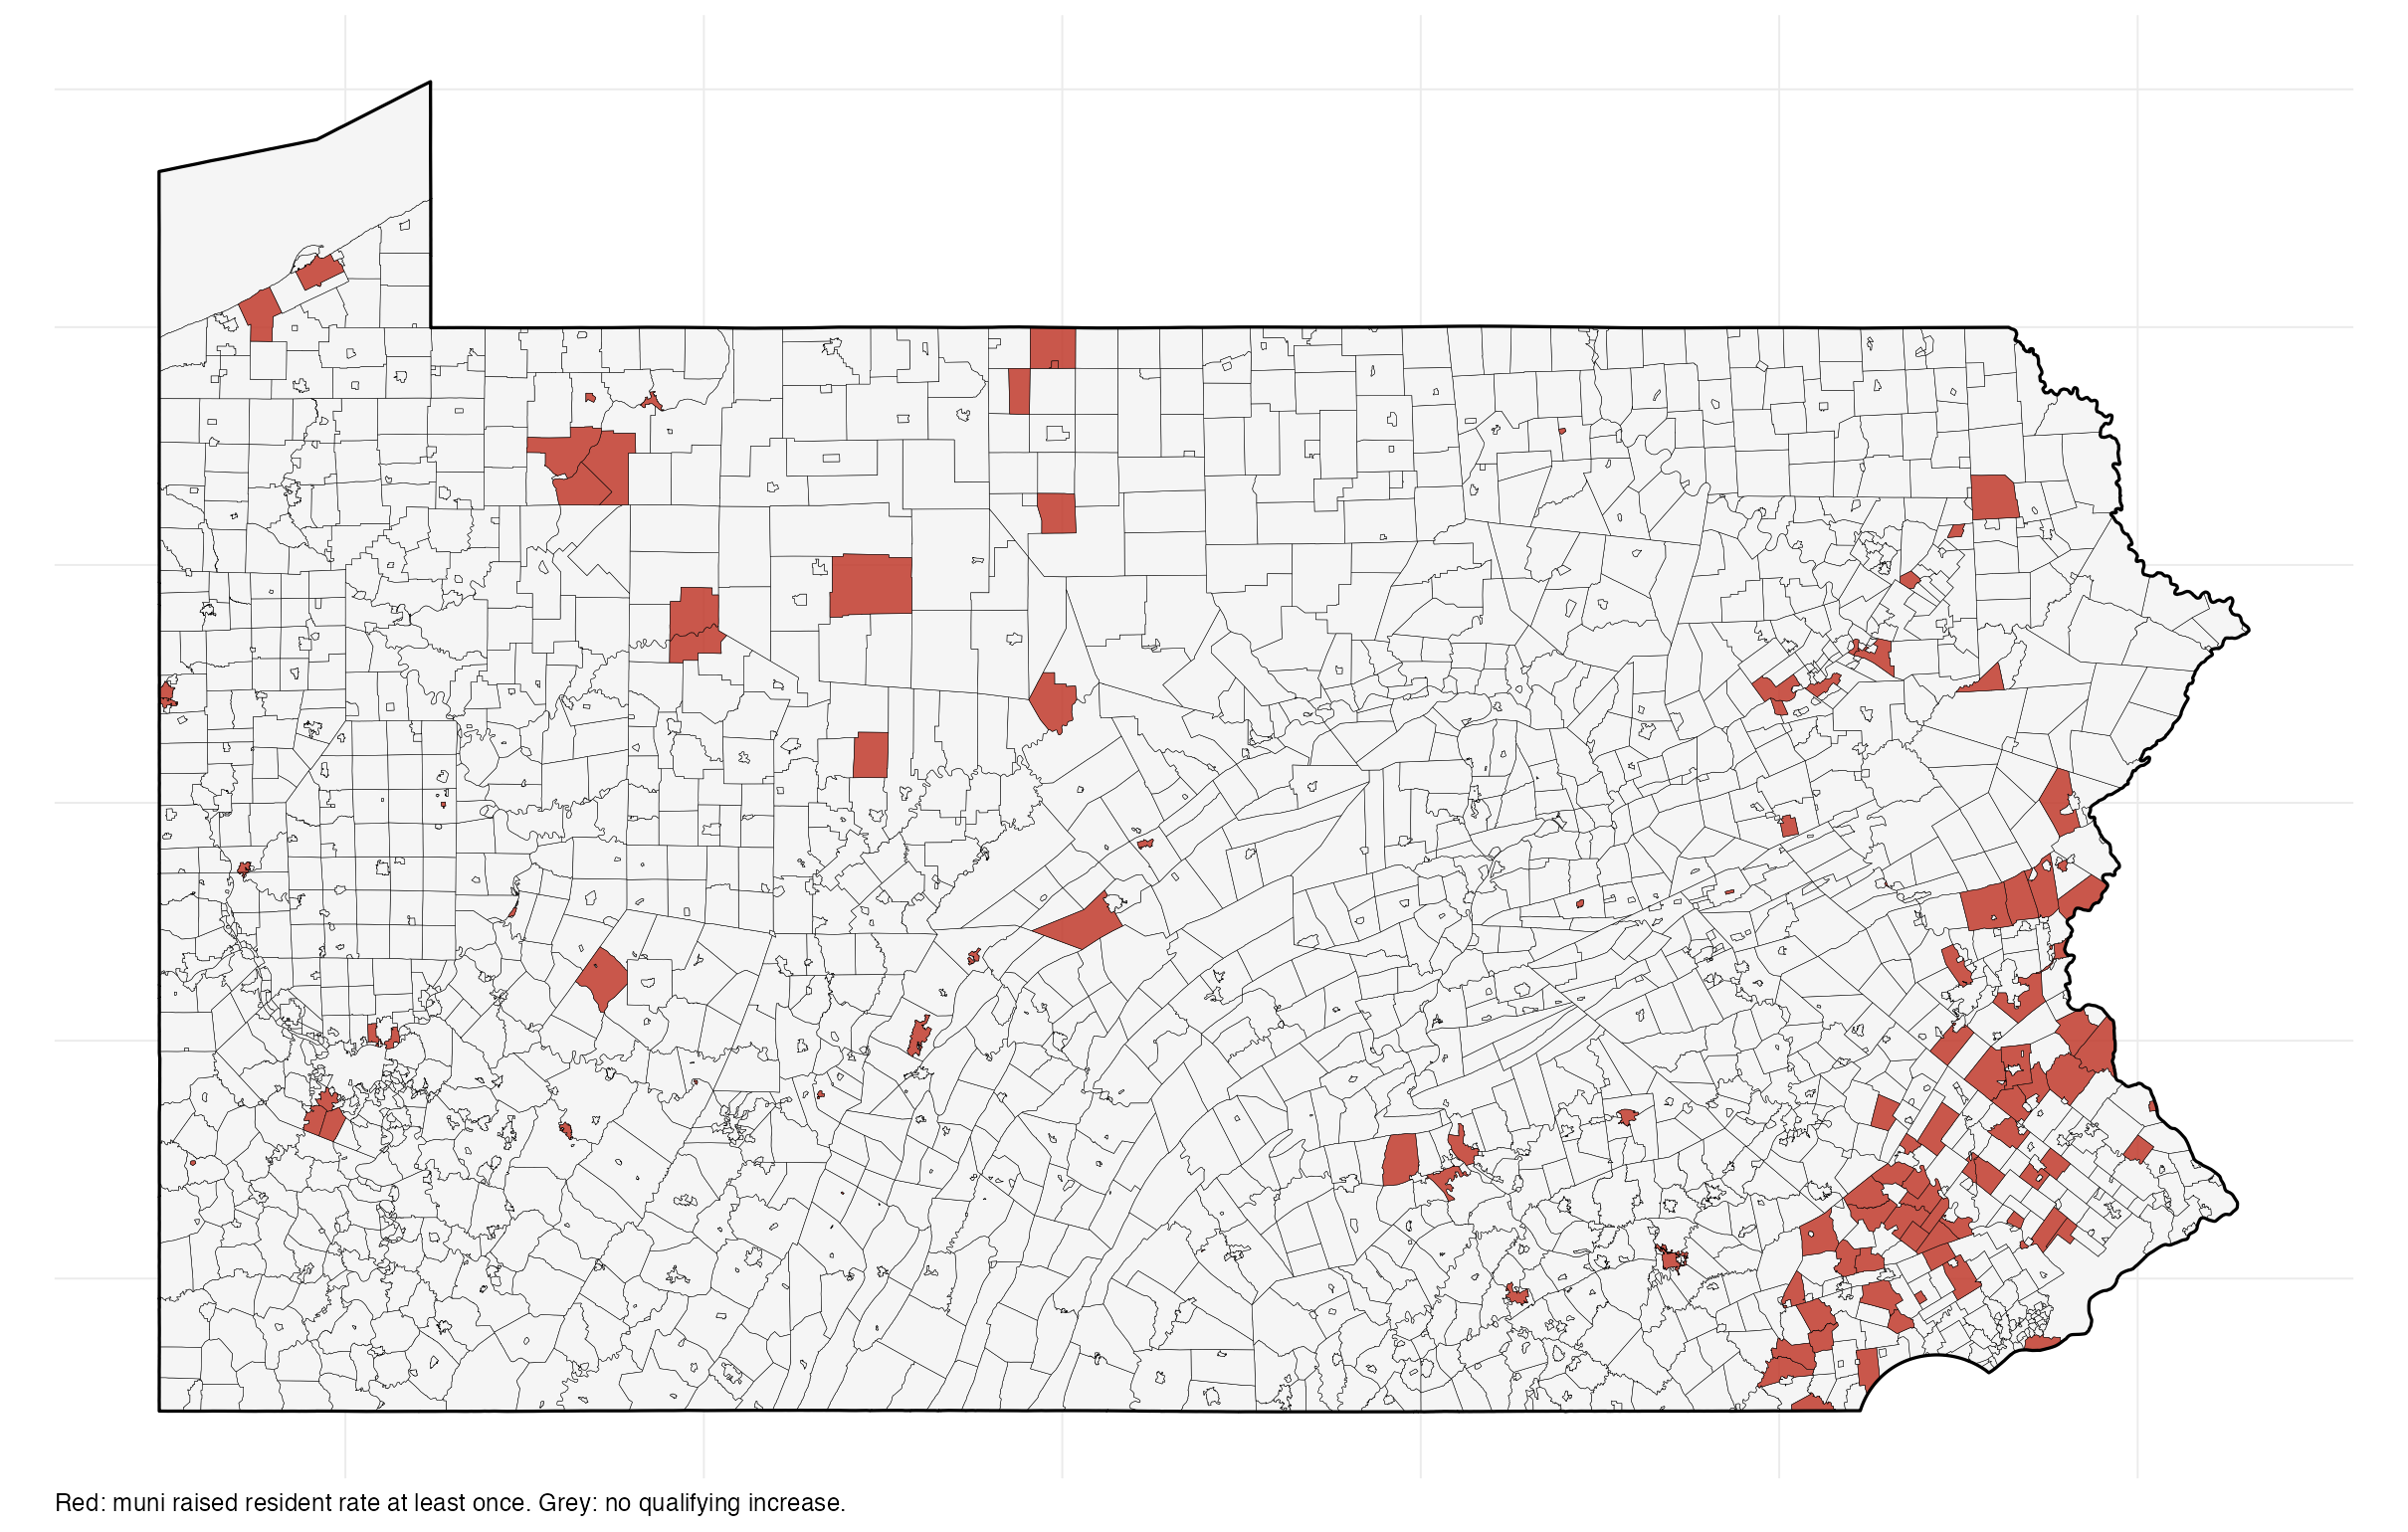
\includegraphics[width=0.85\textwidth]{../figures/pa_map.png}
    \caption{Pennsylvania EIT rate changes, 2000--2019. Red =
    increased; blue = decreased; purple = both; grey = no change.}
    \label{fig:pa_map}
\end{figure}

%==========================================================
\section{Empirical Strategy}
\label{sec:strategy}
%==========================================================

I estimate two specifications using a continuous stacked
difference-in-differences design. First, I run a pooled-Increase
aggregate (\S\ref{subsec:pooled-spec}) that collapses all
rate-increase events at each rate-setter into a single only-increase
group. Second, I estimate a binding
decomposition (\S\ref{subsec:stacked-continuous}) on the three
Increase cells defined in
Section~\ref{sec:theory}, isolating the rate changes that move the
worker's bill from those that do not. Both specifications are
estimated at the municipality-year level. Decrease cells are not estimated: the cohort is
thin ($4$ Dec-bind, $3$ Dec-becomes-non, $11$ Dec-nobind) and the
realized-dose pre-trend rejects parallel trends on every Dec outcome
(Wald $p<0.001$), so the Dec coefficients cannot be interpreted as
causal. Note that a theoretical case for symmetric responses to
rate cuts and rate hikes is weak in any event: moving costs are
sunk, so rate \emph{cuts} are less salient to incumbent residents
than rate hikes (those who would have moved out absent the cut
stay; those who would not have moved in absent the cut do not
necessarily arrive), and the predicted-Dec response is therefore
expected to be smaller and slower than the predicted-Inc response
even with a clean estimating sample. Pre-trends are tested
separately by a realized-dose Sun--Abraham event study
(\S\ref{subsec:pretrend-diagnostics}). Fiscal controls and outcomes
are introduced in Section~\ref{sec:data}; this section focuses on
estimating equations, identification, and diagnostics.


\subsection{Pooled Aggregate Specification}
\label{subsec:pooled-spec}

In this section I report an aggregate specification that pools the
treated Increase cells per rate-setter into a single directional group
$\text{Inc}$ (any rate increase), with
$\text{NC}$ never-changers as the omitted reference. Decrease cells
are excluded for the reasons given in \S\ref{sec:strategy}. The pooled
regression answers: what is the average per-percentage-point (pp)
effect of a rate hike on residents, ignoring whether or not the
hike binds? The binding decomposition that follows in
Equation~(\ref{eq:headline}) then explains which sub-population of
the treated municipality cohort drives the pooled coefficient.

For each unit-time observation $(i, t)$ on the stacked panel, the
per-pp pooled regression is

\begin{equation}
\begin{split}
Y_{\tilde i \tilde t} \;=\; \alpha_{\tilde i} \;+\; \gamma_{\tilde t}
&+ \beta^{M}_{\text{Inc}}\;\Delta\tau^{M}_{it}\,\mathbf{1}\!\left\{d^{M}_{i} = \text{Inc}\right\} \\
&+ \beta^{SD}_{\text{Inc}}\;\Delta\tau^{SD}_{it}\,\mathbf{1}\!\left\{d^{SD}_{i} = \text{Inc}\right\} \\
&+ \mathbf{X}'_{it}\boldsymbol{\phi}
\;+\; \varepsilon_{\tilde i \tilde t}.
\end{split}
\label{eq:pooled}
\end{equation}

The dependent variable $Y_{\tilde i \tilde t}$ is the outcome of
interest. At the municipality level the
outcomes are the logs of live-and-work workers (residents employed
in their own municipality), in-commuters, out-commuters, total jobs, and
total residents, plus the share of workers living in their own
municipality, the share of workers who are nonresidents, and the share of
residents working outside the municipality. The unit $i$ is a municipality. The subscripts $\tilde i = (i, c)$ and
$\tilde t = (t, c)$ are the unit-by-stack and year-by-stack
groupings where each treated unit $i$ appears in exactly one
sub-experiment (its first-event cohort $c$), while each NC unit
appears in every cohort it overlaps. Cohort $c$ is defined as the first year that the rate-setter changed $\tau$. The fixed effects
$\alpha_{\tilde i}$ and $\gamma_{\tilde t}$ are for each unit and cohort pair. The directional grouping
$d^{s}_{i} \in \{\text{NC}, \text{Inc}\}$ classifies
unit $i$'s rate trajectory on rate-setter $s \in \{M, SD\}$, with
NC the omitted reference as they are the control group. The
dose $\Delta\tau^{s}_{it} = \tau^{s}_{it} - \tau^{s}_{i, c-1}$ is
the cumulative change in the rate from the pre-event baseline
($c-1$, one year before the first event) to year $t$, measured in
percentage points; it is zero in pre-event years and for NC units,
and accumulates with subsequent rate changes within $i$. The control vector
$\mathbf{X}_{it}$ holds the six municipality fiscal share controls
(police-services, streets, debt-service, EIT-revenue,
real-estate-tax, intergovernmental-revenue).
$\boldsymbol{\phi}$ is the
coefficient vector on these controls and $\varepsilon_{\tilde i \tilde t}$
is the residual.

\subsection{Binding Decomposition: Stacked Continuous DiD}
\label{subsec:stacked-continuous}

The binding decomposition is the main estimator of the paper. It
replaces the two-level direction grouping $d^s_i$ from
Equation~\ref{eq:pooled} with a multilevel cell
$\text{cell}^s_i$ that entails both the direction of unit $i$'s
first event and whether the home stack was binding pre- and
post-event (Section~\ref{subsec:cells}, Table~\ref{tab:cells}).
This splits the increase side into Inc-bind, Inc-becomes, and
Inc-nobind; NC remains the omitted reference. Decrease cells are
not estimated for the reasons discussed in
\ref{sec:strategy}. The stacked
panel, unit-by-stack groupings, dose $\Delta\tau^s_{it}$, controls
$\mathbf{X}_{it}$, fixed effects, and policy-jurisdiction
clustering are identical to Equation~\ref{eq:pooled}. The
sub-experiment for each cohort $c$ runs on the window
$t \in [c-K, c+K]$ with $K=5$, which gives the realized-dose ES
diagnostic four pre-event leads (Section~\ref{subsec:pretrend-diagnostics})
and covers the bulk of the treated units with a full $5$-pre,
$5$-post window.

For each rate-setter $s$ and outcome $Y$ the stacked-continuous
regression is

\begin{equation}
\begin{split}
Y_{\tilde{i}\tilde{t}} \;=\; \alpha_{\tilde{i}} \;+\; \gamma_{\tilde{t}}
&+ \sum_{k \in \mathcal{C}_{-\text{NC}}} \beta^{\text{muni}}_k \;\Delta\tau^{\text{muni}}_{it} \cdot \mathbf{1}\{\text{cell}^{\text{muni}}_i = k\} \\
&+ \sum_{k \in \mathcal{C}_{-\text{NC}}} \beta^{\text{SD}}_k  \;\Delta\tau^{\text{SD}}_{it}   \cdot \mathbf{1}\{\text{cell}^{\text{SD}}_i = k\}   \\
&+ \mathbf{X}'_{it}\boldsymbol{\phi}
\;+\; \varepsilon_{\tilde{i}\tilde{t}}.
\end{split}
\label{eq:headline}
\end{equation}

The set
$\mathcal{C}_{-\text{NC}} = \{\text{Inc-bind, Inc-becomes, Inc-nobind}\}$
collects the three estimated treated cells; $\text{cell}^s_i$ is the cell label
on rate-setter $s$ and the unit level being modeled $i$. The regression returns three $\beta^s_k$
coefficients per rate-setter, each the per-pp dose-response of $Y$
to a 1 pp change in rate $s$ restricted to units in cell $k$, with
NC units on the same rate-setter as controls. The
$\beta^{\text{muni}}_{\text{Inc-nobind}}$ coefficient is the
within-design placebo meaning that the rate hike
does not move the worker's bill in this cell, so the coefficient
should be statistically indistinguishable from zero. All other
elements of the regression are inherited from
Equation~\ref{eq:pooled}.

The construction uses the negative-weighting fix from
\citet{goodman-baconDifferenceindifferencesVariationTreatment2021}:
treated units enter exactly one stack (their first-event cohort),
NC units enter every stack, so no treated unit serves as control
to a later-treated unit. The cell decomposition is a
novel additional because it generates a ladder of predictable effects including the within-design placebo
(Inc-nobind), which the pooled stacked DiD
classification cannot produce.

The identifying variation in this design comes from the cross-unit cumulative rate changes after each unit's first
event. Figure~\ref{fig:dose_trajectory} and Figure~\ref{fig:dose_trajectory_inc_becomes}
show the average change post event by rate-setter. Each line plots the cross-muni mean and
inter-quartile range of cumulative $\Delta\tau$ at each event-time. Figure~\ref{fig:dose_trajectory}
traces the mean cumulative resident-rate change of Inc-bind units relative to their pre-event baseline. The
pre-event window is mechanically flat at zero by construction (dose
is measured relative to the unit's own $c-1$ rate) and the post-event
window shows the realized cumulative $\Delta\tau^{\text{muni}}$
rising to roughly $0.20$ percentage points by $k = +5$. While the school district rate sits far above the municipal rate at roughly $0.60$ percentage points.


\begin{figure}[H]
  \centering
  \caption{Cumulative Inc-bind dose by event-time: municipality cohort vs.\ school-district cohort.}
  \label{fig:dose_trajectory}
  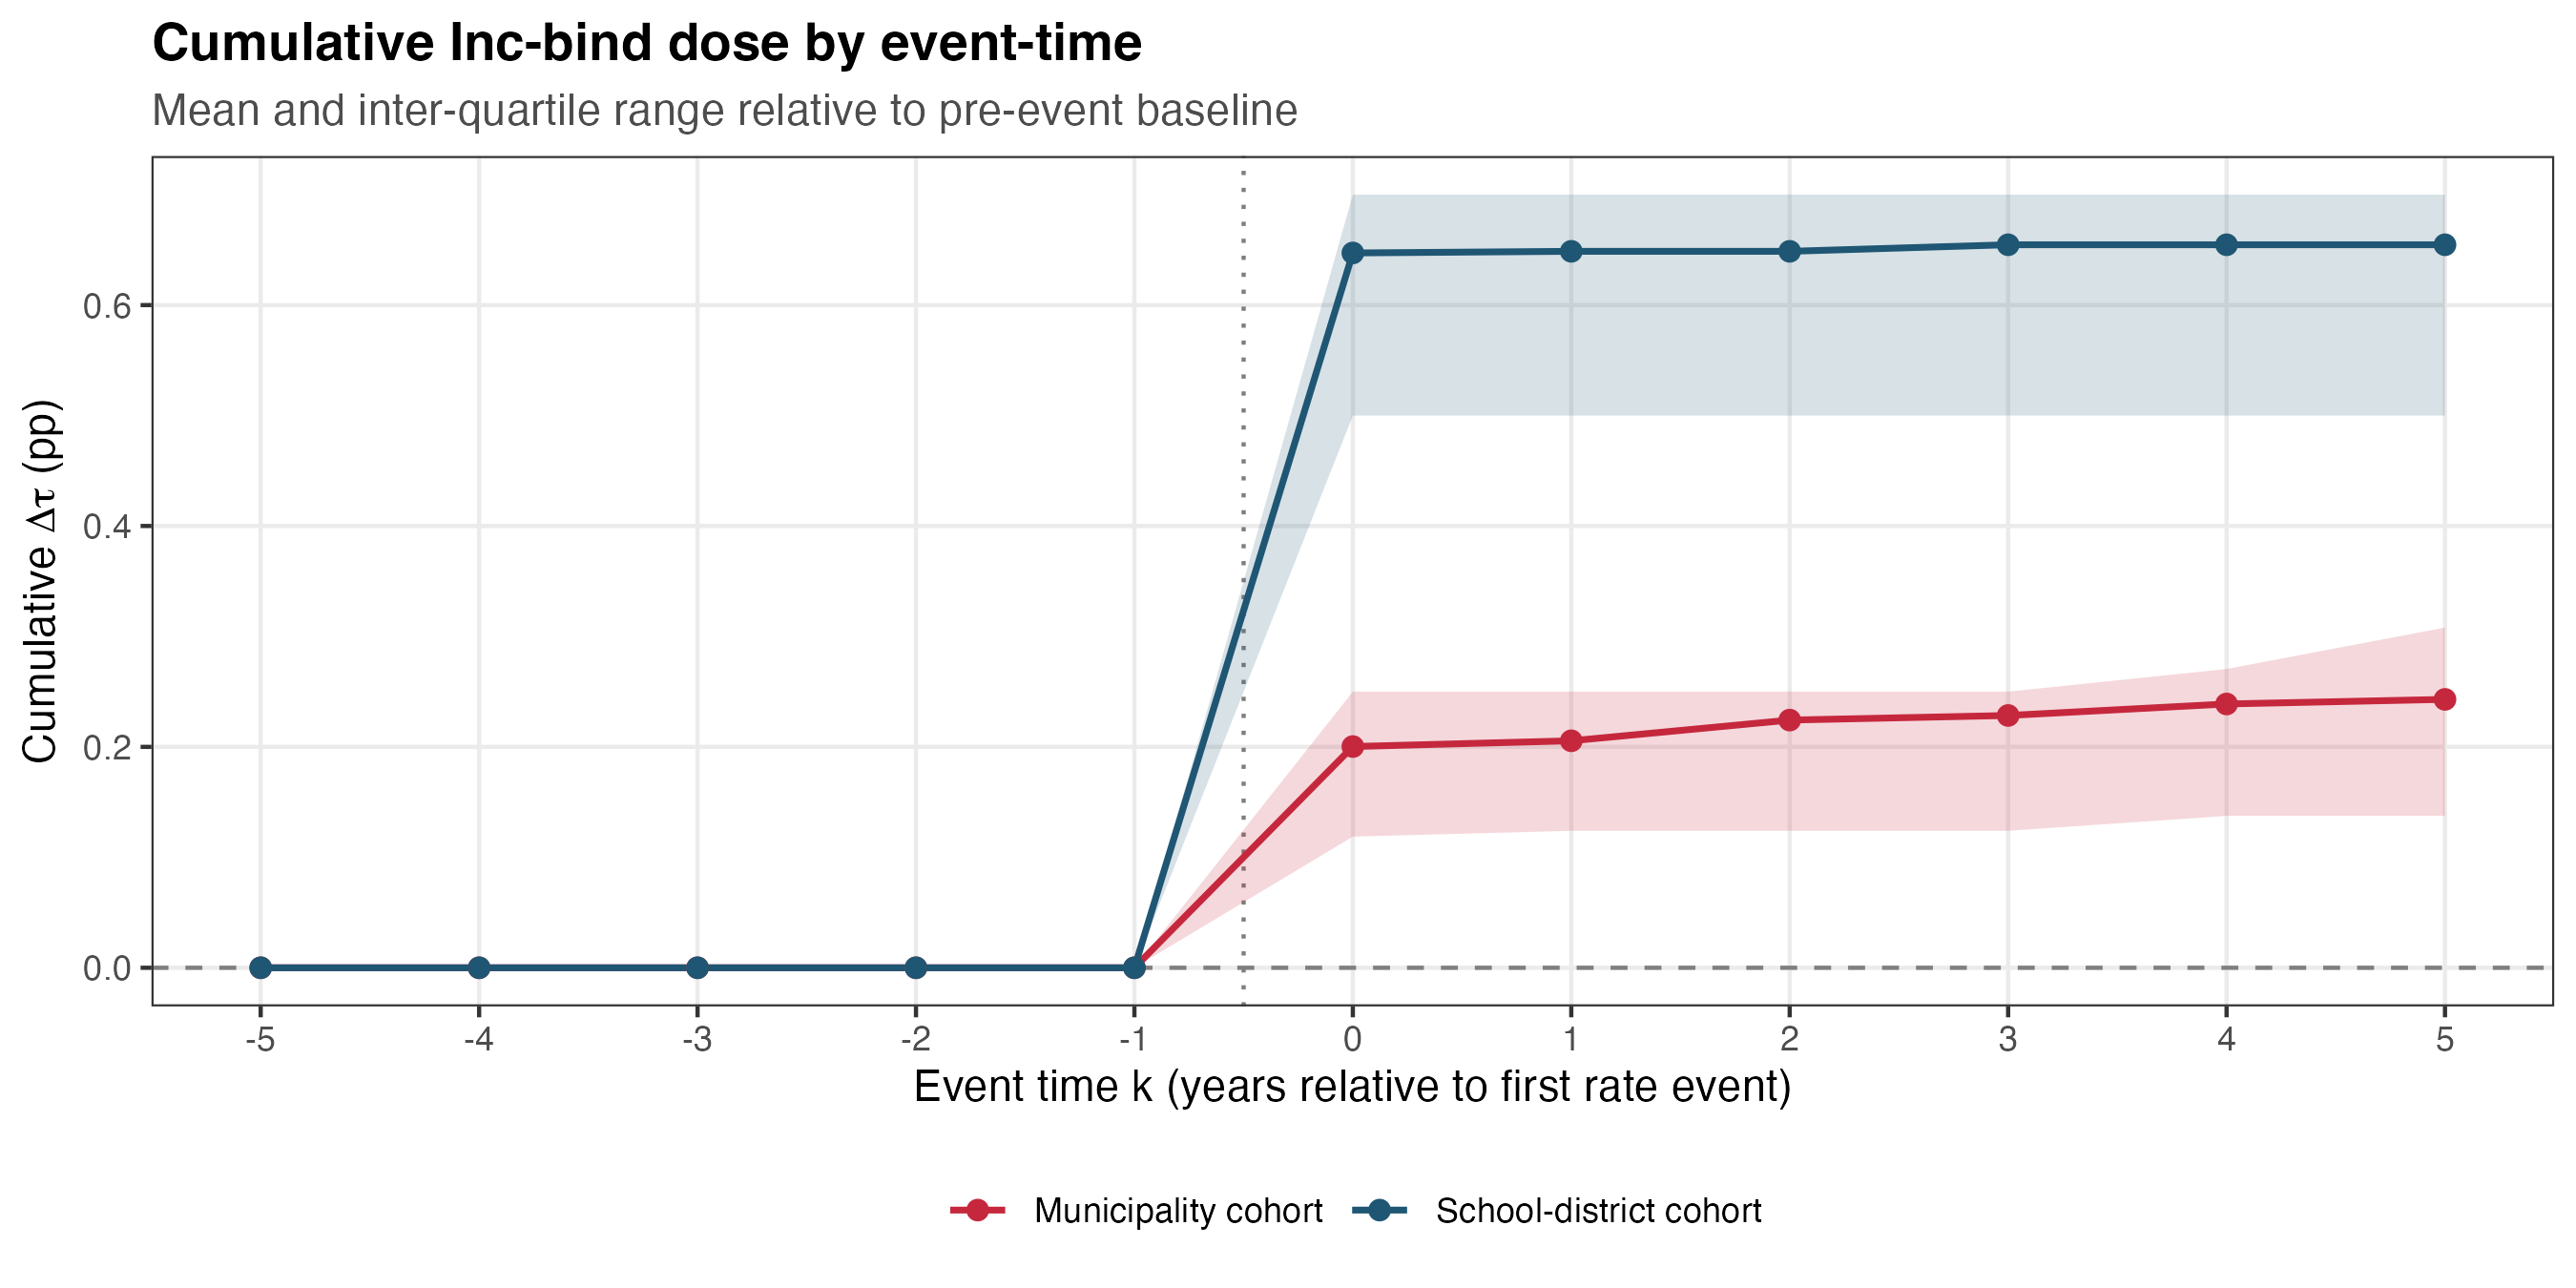
\includegraphics[width=0.85\textwidth]{../figures/support_dose_trajectory_muni_vs_sd.png}
  \begin{minipage}{0.85\textwidth}
    \footnotesize \textit{Notes:} Mean and inter-quartile range of
    cumulative dose by relative event-time $k$. The municipality
    cohort (red) reaches a mean of $0.24$ pp at $k=+5$; the
    school-district cohort (blue) reaches $0.65$ pp. Pre-event
    values are zero by construction.
  \end{minipage}
\end{figure}

Figure~\ref{fig:dose_trajectory_inc_becomes}
traces the mean cumulative resident-rate change of Inc-becomes binding on units relative to their pre-event baseline. The post-event
window shows a similar effect as figure~\ref{fig:dose_trajectory} where the school district rates sit above municipality rates at $0.60$ percentage points but the municipality rate above $0.40$ and is a much larger increase and the gap between the average school district and average municipality rate changes is smaller. Figure~\ref{fig:dose_trajectory_inc_becomes} indicates that for an the rate to become binding the jump may primarily due to municipality rate adjustments.

\begin{figure}[H]
  \centering
  \caption{Cumulative Inc-becomes dose by event-time: municipality cohort vs.\ school-district cohort.}
  \label{fig:dose_trajectory_inc_becomes}
  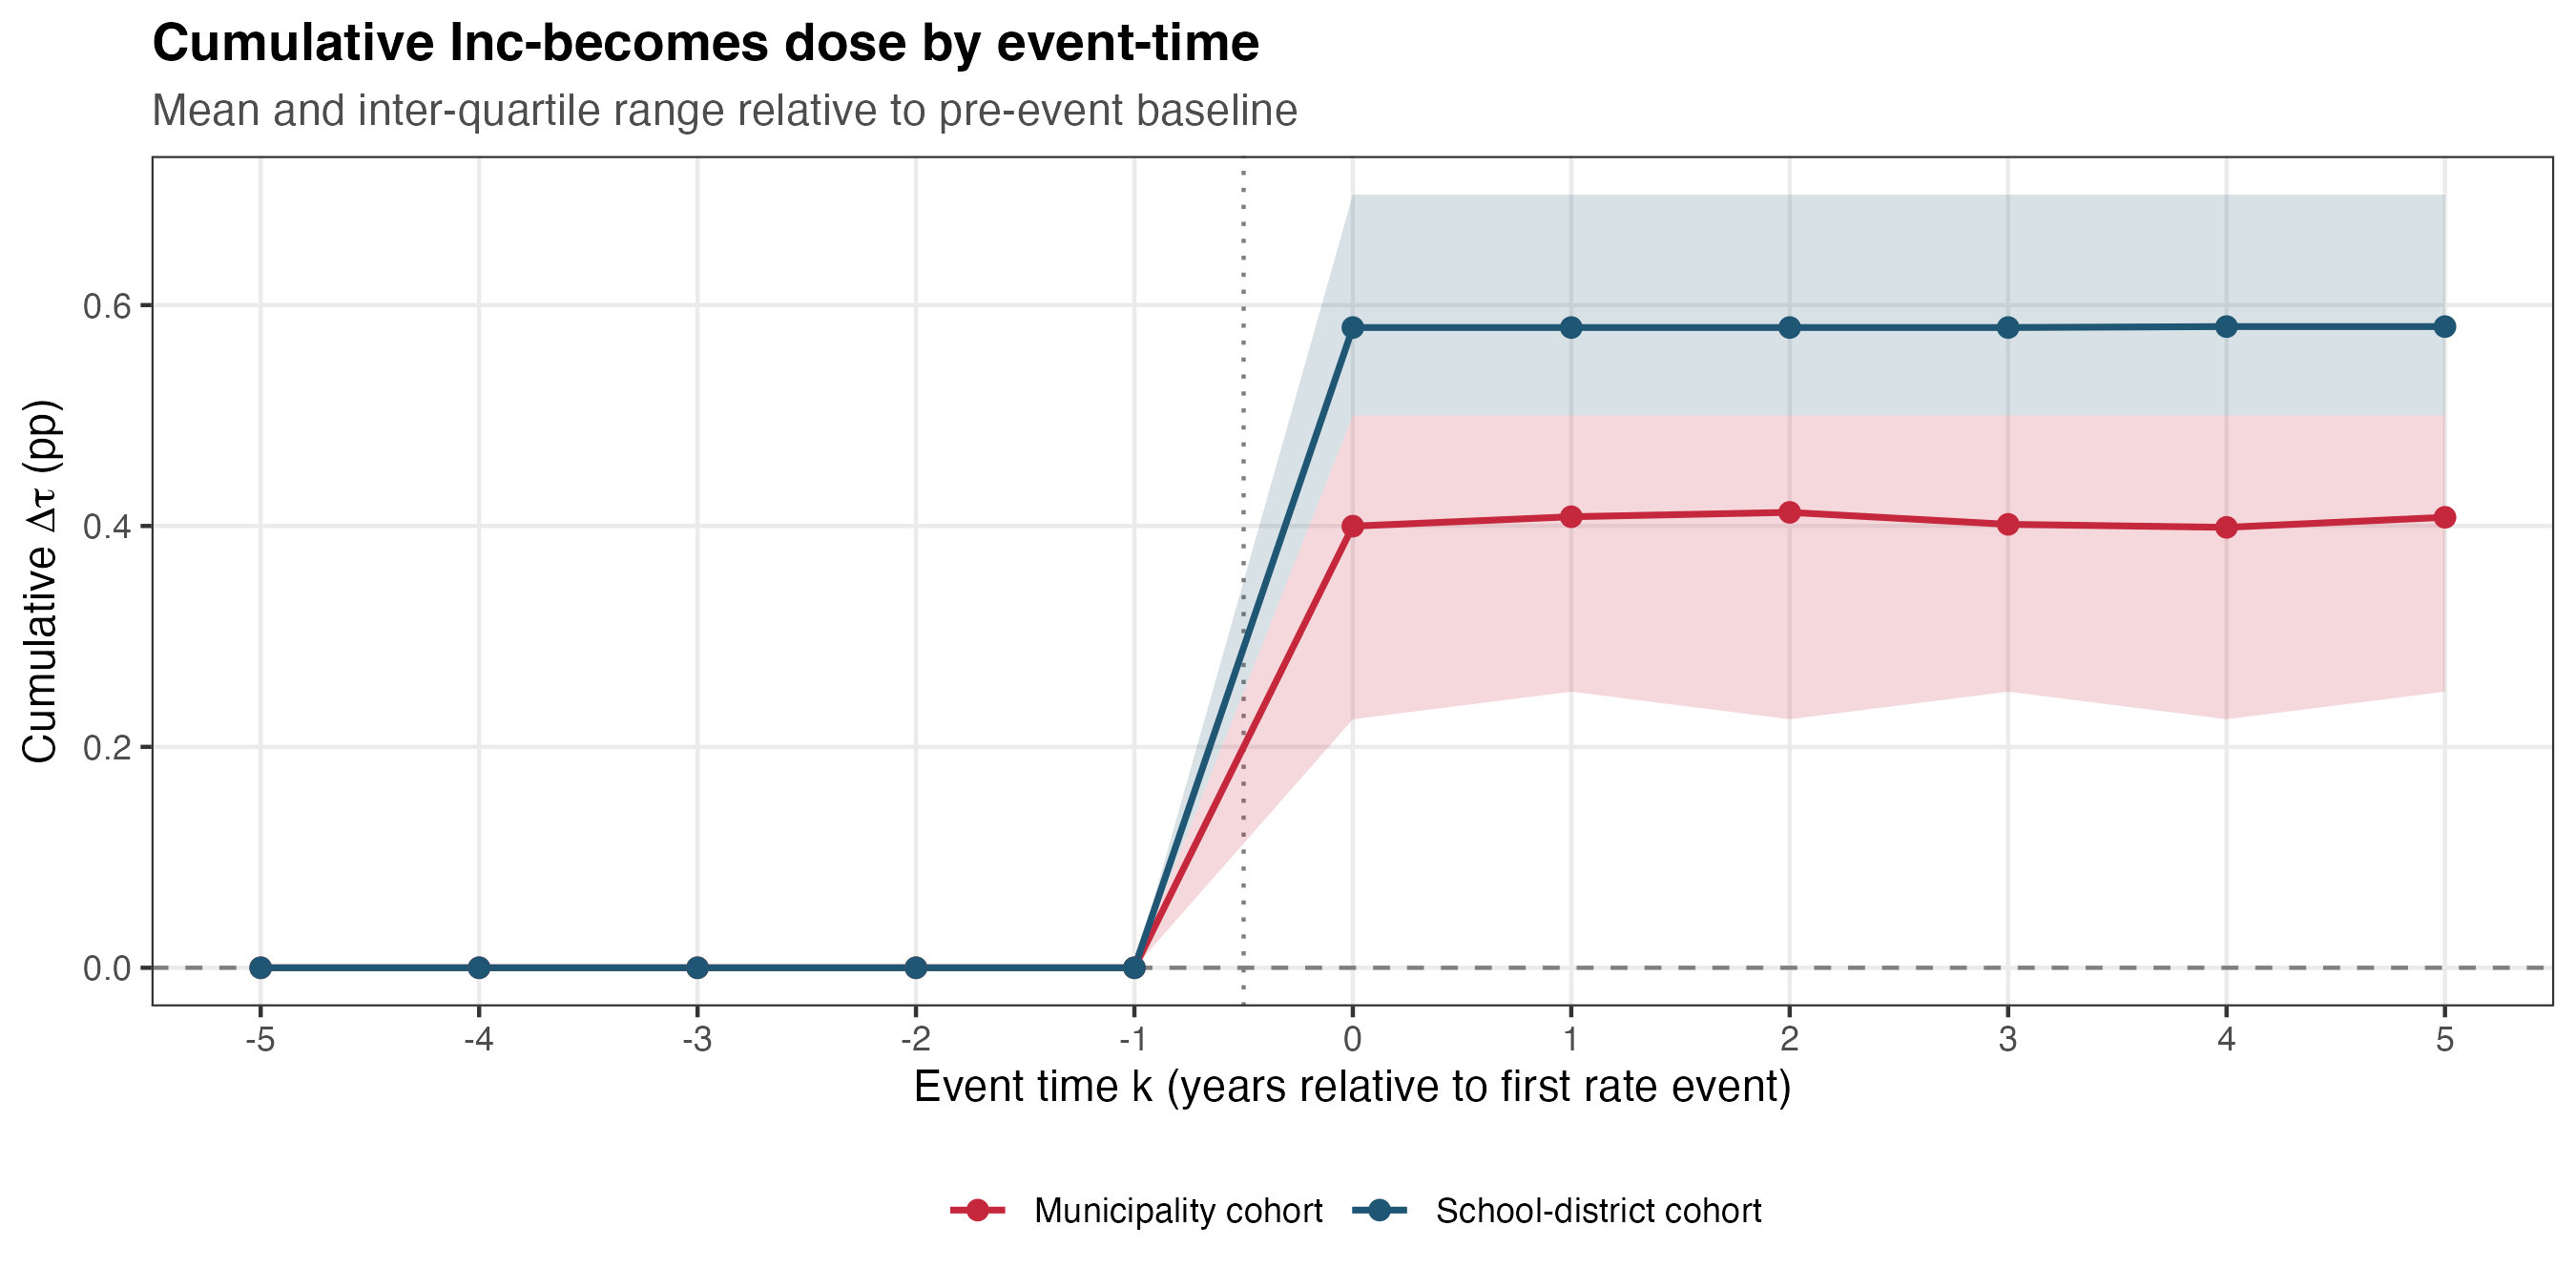
\includegraphics[width=0.85\textwidth]{../figures/support_dose_trajectory_inc_becomes.png}
  \begin{minipage}{0.85\textwidth}
    \footnotesize \textit{Notes:} As in Figure~\ref{fig:dose_trajectory}
    but for the Inc-becomes cell, where the home stack flips from
    non-binding to binding at the first event.
  \end{minipage}
\end{figure}

\subsection{Realized-Dose Event-Study Diagnostic}
\label{subsec:pretrend-diagnostics}
\label{subsec:realized-dose-es}

Equation~\ref{eq:headline} cannot test for pre-treatment leads
directly because $\Delta\tau^s_{it}$ is mechanically zero for all
$t < c$, so any pre-event coefficient on the dose
is also mechanically zero. I therefore run a separate
realized-dose Sun--Abraham event study on the same stacked panel
to test parallel trends, the condition recommended
for continuous-treatment DiD designs by
\citet{callaway2021} and
\citet{dechaisemartin2024} states that units with
larger eventual rate changes should not be on differentially sloped
pre-event trajectories relative to NC controls. For each cell on
rate-setter $s$ I restrict the panel to units in (NC, cell) and
run

\begin{equation}
Y_{it} = \alpha_{\tilde i} + \gamma_{\tilde t}
+ \sum_{k \neq -1} \beta^M_k\, \mathbf{1}\{\ell_{it} = k\}\,
\widetilde{D}_i
+ \mathbf{X}'_{it}\boldsymbol{\phi} + \varepsilon_{it}.
\label{eq:realized-dose-es}
\end{equation}

Two variables are new relative to Equation~\ref{eq:headline}. The
event-time index $\ell_{it} = t - c^M_i$ counts the number of years
between calendar year $t$ and unit $i$'s first muni-rate event,
with $\ell = -1$ (one year before the event) as the omitted
reference. The realized-dose tag
$\widetilde{D}_i = \tau^M_{i, c+5} - \tau^M_{i, c-1}$ is unit $i$'s
cumulative rate change at $k=+5$, measured as observed tax rates which is
unlike $\Delta\tau^s_{it}$ in Equation~\ref{eq:headline}. The units therefore have constant tax rates within unit and varies across treated units in proportion
to eventual treatment intensity, so the per-pp dose-response shows
up in pre-event years even though the rate itself has not yet
moved. The outcome $Y_{it}$, the unit-by-stack and year-by-stack
fixed effects, the control vector $\mathbf{X}_{it}$, the units of
observation, and the policy-jurisdiction clustering are the same
as in Equation~\ref{eq:headline}.

The pre-event coefficients $\beta^M_k$ for $k \leq -2$ are the
parallel-trends test: if units that eventually take large rate
changes are on differentially sloped trajectories before the rate
change, the $\beta^M_k$ at pre-event leads will be non-zero. Under
strong parallel trends they are zero. The post-event coefficients
$\beta^M_k$ for $k \geq 0$ recover the per-pp dose-response at
each event-time and average to the corresponding cell coefficient
$\beta^s_{\text{cell}}$ from Equation~\ref{eq:headline} when the
unit's rate path is a single step at the event year. I report the
joint Wald $p$-value across $k \leq -2$ as a single pre-trend
statistic for each cell-outcome combination.

Section~\ref{sec:results} reports the headline binding
decomposition at each estimating unit and the pooled-Increase
benchmark. Auxiliary diagnostics (pre/post Act~32 split, Act~47
exclusion) are in Section~\ref{sec:robustness}.


%==========================================================
\section{Results}
\label{sec:results}
%==========================================================

I report results in two layers. First,
Section~\ref{subsec:results-pooled} presents the pooled Inc
benchmark, which approximates what a conventional local-tax design
would recover by averaging across all rate-increase events without
distinguishing whether they bind. Second,
Section~\ref{subsec:results-decomp} reports the binding
decomposition at the municipality level. The central empirical
comparison is between the Inc-bind cell (where the statutory rate
change moves the worker's bill) and the Inc-nobind cell (where it
does not), with Inc-nobind serving as the within-design placebo.
Dec cells are not estimated: the cohort is thin
(4 Dec-bind, 3 Dec-becomes-non, 11 Dec-nobind) and the
realized-dose pre-trend rejects parallel trends on every Dec
outcome (Wald $p<0.001$), so the Dec coefficients cannot be
interpreted as causal. The pre-/post-Act-32 enforcement-break split
appears in the Robustness section.

\subsection{Pooled-Increase Benchmark}
\label{subsec:results-pooled}

I first report the pooled-Increase specification from
Equation~(\ref{eq:pooled}), which collapses each rate-setter to a
single direction tag for rate increases. The pooled coefficients
are useful because they approximate the estimand in a conventional
local-tax design: the average per-pp dose-response of a
municipality-rate change and an SD-rate change without
distinguishing whether the rate change moves the worker's bill.

Table~\ref{tab:pooled_per_pp_cousub} reports the per-pp pooled
coefficients at the municipality level. The table reports the two
coefficients of interest per outcome: the municipality resident-rate
Inc effect $\beta^M_{\text{Inc}}$ and the school-district-rate Inc
analogue $\beta^{SD}_{\text{Inc}}$.

\begin{table}[H]
  \centering
  \caption{Pooled Inc/Dec headline --- municipality level (per pp)}
  \label{tab:pooled_per_pp_cousub}
  \small
  \resizebox{\textwidth}{!}{
  \begin{tabular}{lcccc}
    \toprule
    Outcome & Log(work in own muni) & Log(in-commuters) & Log(employed residents) & Share live in muni \\
    \midrule
    \textbf{Municipality rate ($\tau^{M}$)} & & & & \\
    \quad $\Delta\tau > 0$ (Inc) & -0.228\sym{***} & -0.209\sym{***} & -0.035 & -0.019\sym{**} \\
                           & (0.058) & (0.056) & (0.033) & (0.008) \\
    \quad $\Delta\tau < 0$ (Dec) & 0.260\sym{**} & 0.014 & 0.058 & 0.022 \\
                           & (0.107) & (0.143) & (0.138) & (0.019) \\
    \textbf{School district rate ($\tau^{SD}$)} & & & & \\
    \quad $\Delta\tau > 0$ (Inc) & 0.128\sym{*} & 0.105 & 0.051 & 0.007 \\
                           & (0.070) & (0.067) & (0.038) & (0.005) \\
    \quad $\Delta\tau < 0$ (Dec) & -0.310\sym{***} & -0.170\sym{**} & 0.020 & -0.003 \\
                           & (0.110) & (0.076) & (0.051) & (0.007) \\
    \midrule
    $N$ & 218,677 & 239,023 & 242,722 & 239,033 \\
    $R^2$ & 0.964 & 0.959 & 0.981 & 0.823 \\
    Within $R^2$ & 0.001 & 0.001 & 0.001 & 0.001 \\
    Dep.\ mean & 3.677 & 5.847 & 6.697 & 0.093 \\
    Dep.\ SD & 1.934 & 1.887 & 1.299 & 0.076 \\
    \bottomrule
  \end{tabular}
  }
  \vspace{0.3em}
  \begin{minipage}{0.95\textwidth}
    \footnotesize \textit{Notes:} Cluster-robust standard errors in parentheses. Each regression includes both rate-setters' direction-pooled treatments jointly; the four reported coefficients are $\beta^M_{\text{Inc}}$, $\beta^M_{\text{Dec}}$, $\beta^{SD}_{\text{Inc}}$, $\beta^{SD}_{\text{Dec}}$. $^{*}p<0.10$, $^{**}p<0.05$, $^{***}p<0.01$.
  \end{minipage}
\end{table}


The muni-rate Inc coefficient on log live-and-work is
$-0.232^{**}$; the cell decomposition in
Section~\ref{subsec:results-decomp} shows this aggregate is driven
by Inc-bind ($-0.573^{***}$) with Inc-becomes and Inc-nobind
averaged in. The pooled-Inc ES on log live-and-work fails parallel
trends (Wald $p=0.001$; Table~\ref{tab:es_pooled_cousub}) because
Inc-becomes and Inc-nobind munis enter with non-zero pre-event
trajectories. The Inc-bind cell on its own passes pre-trends
cleanly ($p=0.33$; Section~\ref{subsubsec:decomp-es}), which is
why the decomposition rather than the pooled coefficient carries
the causal claim. The SD-rate Inc coefficient on the same outcome
is $+0.177^{*}$ and sign-reversed: aggregating across an SD mixes
the rate-changing municipality (where residents may move out) with
non-changing munis in the same SD (which may gain residents from
within-SD movers).

\subsubsection{Realized-dose ES benchmark diagnostic}
\label{subsubsec:pooled-es}

Table~\ref{tab:es_pooled_cousub} reports the ATT summary of the
muni-level pooled realized-dose event study, with the
cluster-robust Wald pre-trend $p$-value for the joint null
$\beta_k = 0$ at $k \leq -2$.
Figure~\ref{fig:pooled_es_muni_only} plots the event-time path.

\begin{table}[!htbp]
  \centering
  \caption{Pooled realized-dose event study --- municipality level.}
  \label{tab:es_pooled_cousub}
  \footnotesize
  \renewcommand{\arraystretch}{0.85}
  \resizebox{\textwidth}{!}{
  \begin{tabular}{lcccc}
    \toprule
    Direction & Log(work in own muni) & Log(in-commuters) & Log(employed residents) & Share live in muni \\
    \midrule
    \textbf{Inc} (post) & -0.232 & -0.254 & -0.029 & -0.014 \\
                      & (0.039) & (0.039) & (0.020) & (0.005) \\
    \textbf{Inc} (pre) & 0.068 & 0.069 & -0.004 & 0.002 \\
                      & (0.032) & (0.055) & (0.038) & (0.007) \\
    \textbf{Inc} Wald $p$ & 0.0012 & 0.0454 & 0.0482 & 0.5333 \\
    \textbf{Dec} (post) & 0.686 & 0.393 & 0.111 & 0.002 \\
                      & (0.207) & (0.126) & (0.045) & (0.006) \\
    \textbf{Dec} (pre) & 0.189 & -0.152 & 0.182 & -0.002 \\
                      & (0.234) & (0.113) & (0.043) & (0.005) \\
    \textbf{Dec} Wald $p$ & $<\!0.0001$ & $<\!0.0001$ & $<\!0.0001$ & $<\!0.0001$ \\
    \midrule
    \multicolumn{5}{l}{\textit{Diagnostics}} \\
    $N$              & 179,169 & 195,702 & 198,654 & 195,711 \\
    $R^2$            & 0.9643 & 0.9605 & 0.9811 & 0.8281 \\
    Within $R^2$     & 0.0013 & 0.0025 & 0.0012 & 0.0016 \\
    Dep.\ mean       & 3.6670 & 5.8570 & 6.6980 & 0.0920 \\
    Dep.\ SD         & 1.9320 & 1.8810 & 1.2960 & 0.0740 \\
    \bottomrule
  \end{tabular}
  }
  \vspace{0.3em}
  \begin{minipage}{0.95\textwidth}
    \footnotesize \textit{Notes:} Cluster-robust standard errors in parentheses. Post = mean of $\beta_k$ for $k = 0, \ldots, 5$; pre = mean for $k \leq -2$. Wald $p$ is the cluster-robust joint test of $H_0\colon \beta_k = 0$ across pre-event $k$. $^{*}p<0.10$, $^{**}p<0.05$, $^{***}p<0.01$.
  \end{minipage}
\end{table}


The pooled-Inc post-event coefficient on log live-and-work is
$-0.257$, with a small but non-zero pre-event lead; the joint Wald
$p=0.002$ rejects strong parallel trends. As above, the rejection
reflects Inc-becomes and Inc-nobind selection rather than a problem
with Inc-bind on its own, which the decomposition isolates.

The other three pooled outcomes shown in
Figure~\ref{fig:pooled_es_muni_only} tell a consistent story.
The pooled-Inc post on log in-commuters is $-0.247$ ($p=0.016$ on
parallel trends), broadly aligned with the live-and-work result.
The pooled-Inc post on log employed residents is much smaller
($-0.045$, $p=0.002$), consistent with the in-commuters response
being broader than residential relocation alone: residents leaving
the muni's labor market entirely or general labor-demand
contraction is part of the channel rather than pure within-CZ
sorting. The share-live-in coefficient is small and negative
($-0.019$, $p=0.14$), and is the only pooled outcome for which
the joint pre-trend test does not reject; share outcomes at the
muni level mix denominator dynamics with binding-channel sorting
and are reported as supporting evidence rather than as primary
identification.

\begin{figure}[H]
  \centering
  \caption{Municipality-level pooled realized-dose event study.}
  \label{fig:pooled_es_muni_only}
  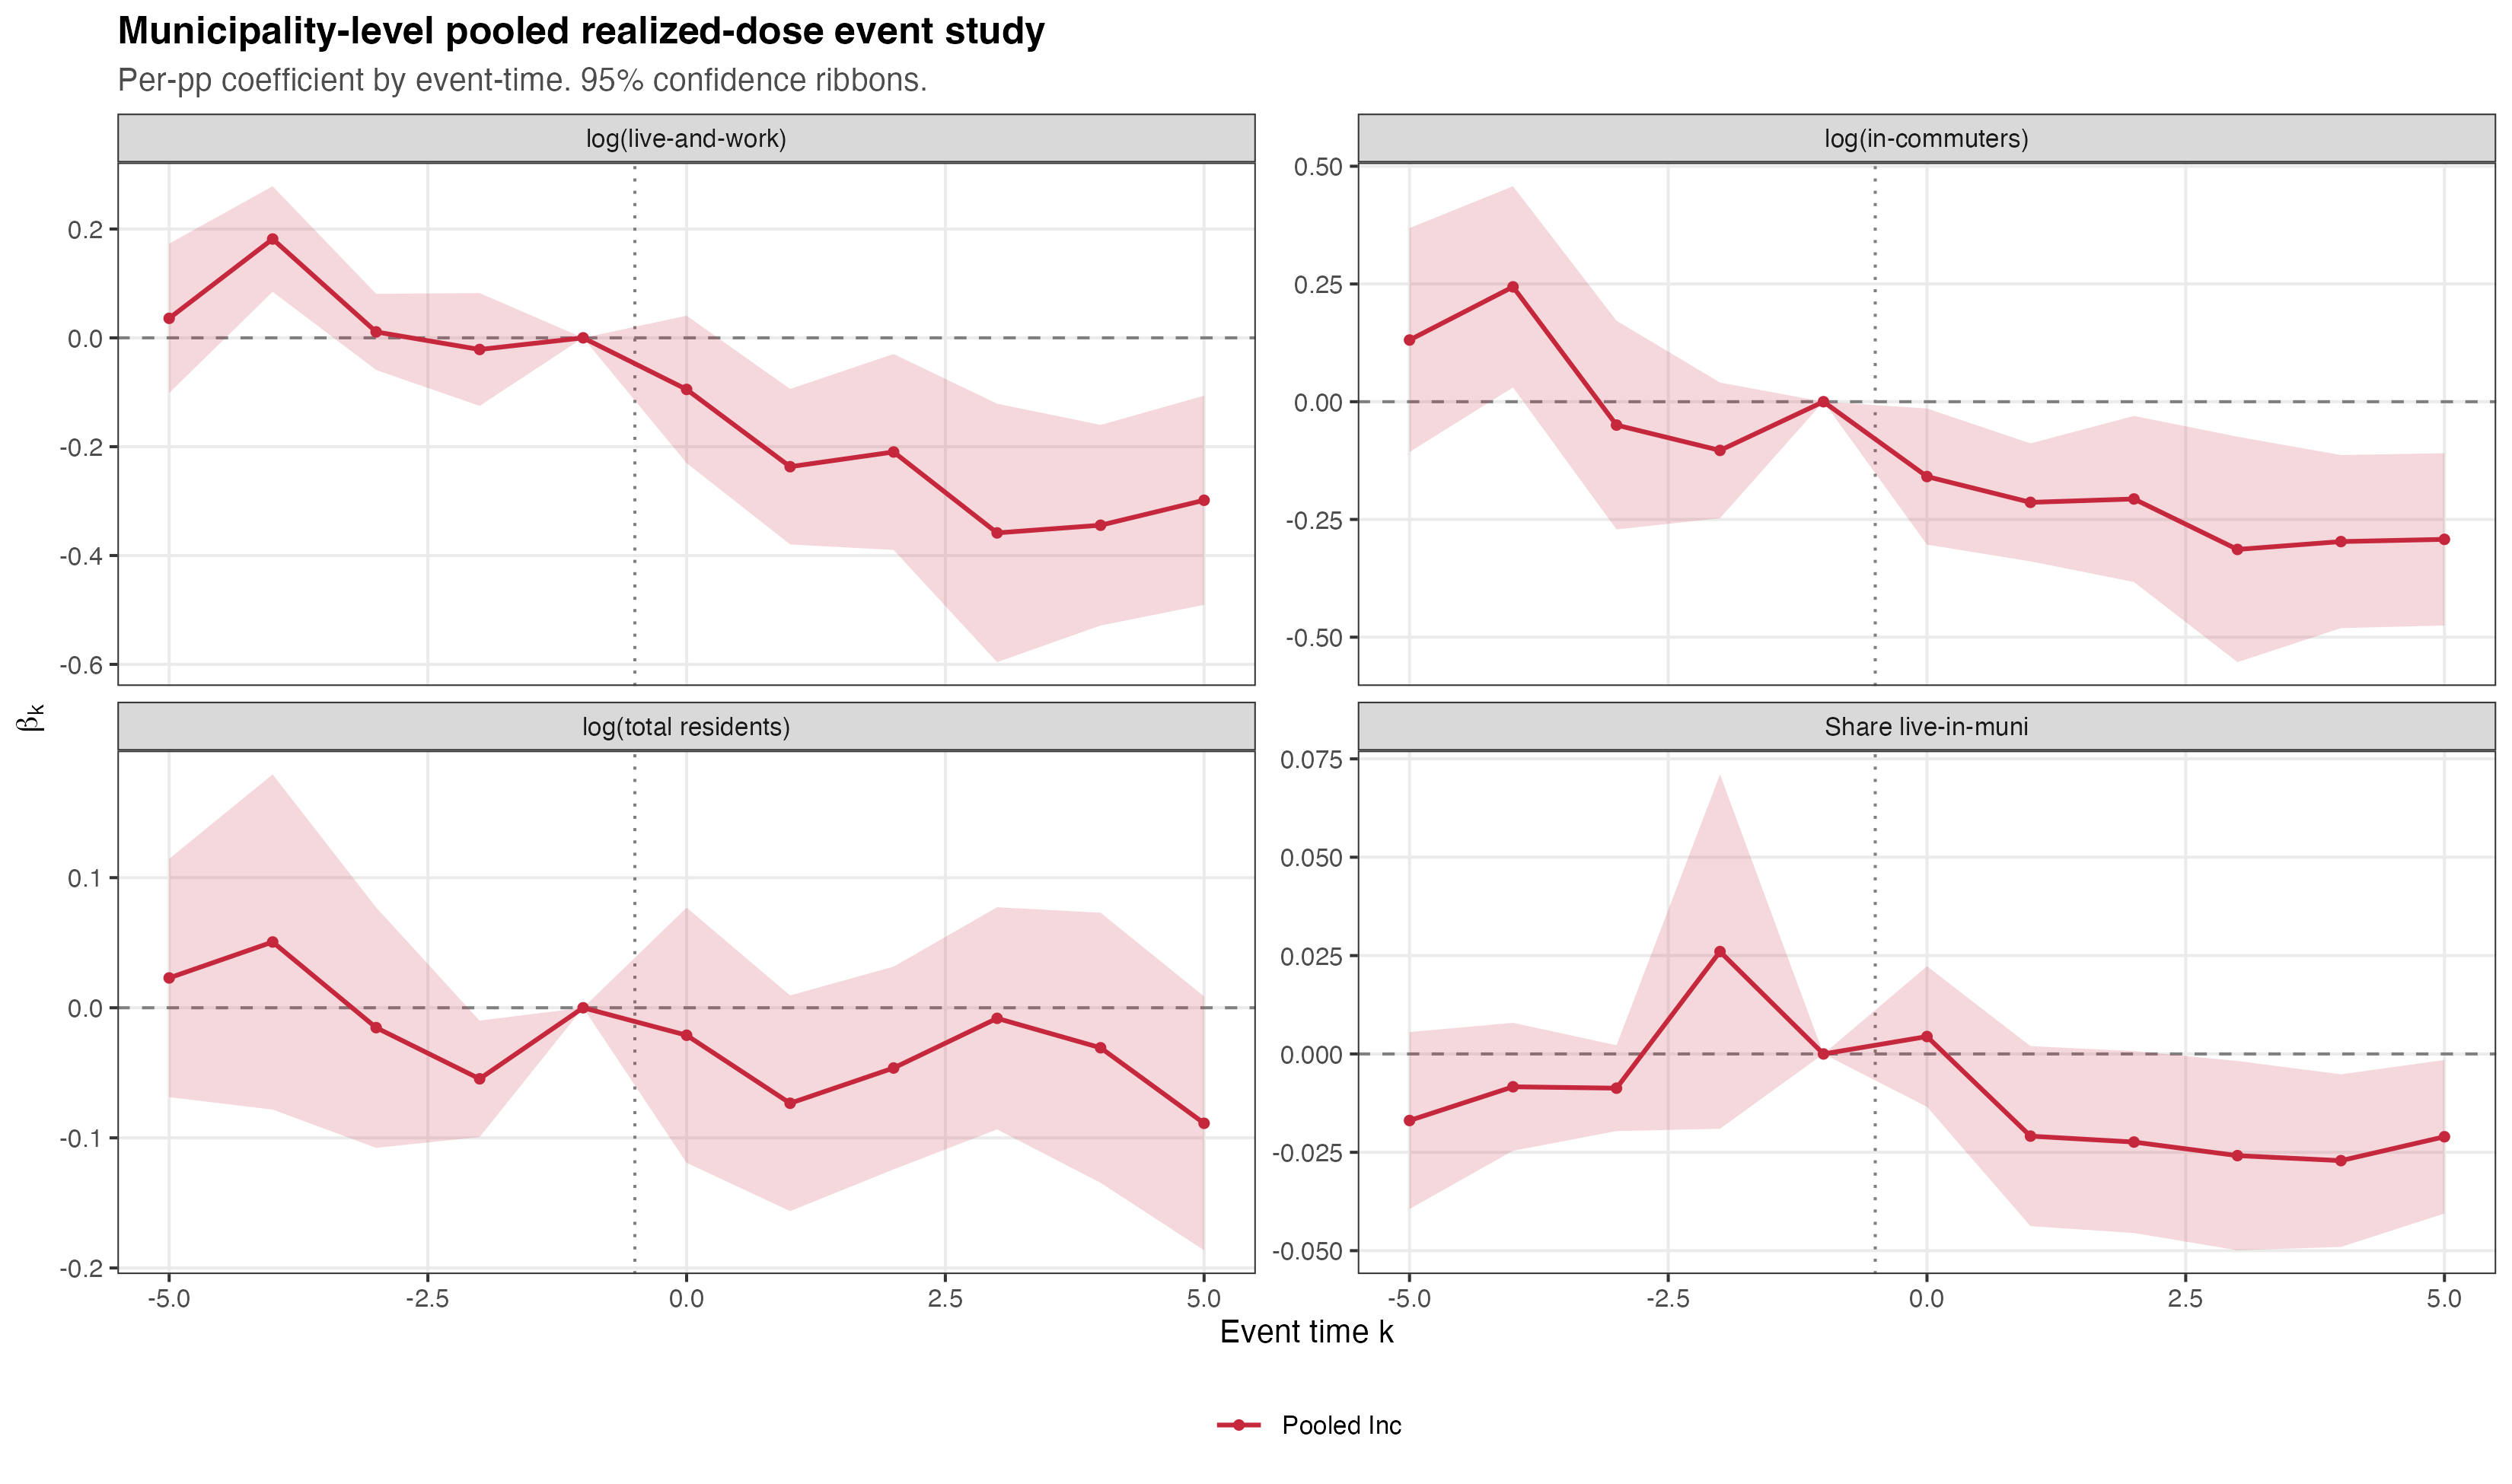
\includegraphics[width=0.95\textwidth]{../figures/pooled_es_muni_only.png}
  \begin{minipage}{0.95\textwidth}
    \footnotesize \textit{Notes:} Per-pp realized-dose coefficient at each event-time for the pooled Inc cohort. Ribbon is the 95\% CI; $k=-1$ omitted as the reference period.
  \end{minipage}
\end{figure}

\subsection{Binding Decomposition}
\label{subsec:results-decomp}
\label{subsec:results-headline}

The decomposition is estimated at the municipality level. Both
rate-setter treatments enter the same joint regression: each
muni-year is assigned its own resident rate $\tau^M$ at native
level and $\max(\tau^{SD})$ across the school districts the muni
reports to (exact for the $97.6\%$ of munis with a single SD,
conservative for the rest). Table~\ref{tab:headline_muni_combined}
reports both sets of cell coefficients from the same joint
regression in a single panel: the muni resident-rate cells (top
panel) are the headline causal claim, and the SD resident-rate
cells (bottom panel) are reported alongside as co-treatment from
the identical specification.

\begin{table}[!htbp]
  \centering
  \caption{Municipality-level dose-response: muni and SD resident-rate cells (joint regression)}
  \label{tab:headline_muni_combined}
  \footnotesize
  \renewcommand{\arraystretch}{0.9}
  \resizebox{\textwidth}{!}{
  \begin{tabular}{lcccc}
    \toprule
    Cell & Log(work in own muni) & Log(in-commuters) & Log(employed residents) & Share live in muni \\
    \midrule
    \multicolumn{5}{l}{\textit{Muni resident rate ($\tau^M$)}} \\
    \textbf{Inc-bind} & -0.573\sym{***} & -0.412\sym{***} & -0.104\sym{**} & -0.058\sym{***} \\
                      & (0.162) & (0.126) & (0.043) & (0.020) \\
    \textbf{Inc-becomes} & -0.250\sym{***} & -0.247\sym{***} & -0.042 & -0.014 \\
                      & (0.056) & (0.055) & (0.027) & (0.011) \\
    \textbf{Inc-nobind} & -0.073 & 0.233 & 0.382\sym{**} & -0.037 \\
                      & (0.143) & (0.302) & (0.188) & (0.032) \\
    \midrule
    \multicolumn{5}{l}{\textit{School district rate ($\tau^{SD}$)}} \\
    \textbf{Inc-bind} & 0.165 & 0.159 & 0.057 & 0.005 \\
                      & (0.109) & (0.096) & (0.049) & (0.007) \\
    \textbf{Inc-becomes} & 0.084 & 0.086 & 0.031 & 0.007 \\
                      & (0.095) & (0.089) & (0.056) & (0.007) \\
    \midrule
    \multicolumn{5}{l}{\textit{Diagnostics}} \\
    $N$           & 174,929 & 191,405 & 194,533 & 191,413 \\
    $R^2$         & 0.963 & 0.959 & 0.980 & 0.825 \\
    Within $R^2$  & 0.001 & 0.001 & 0.001 & 0.001 \\
    Dep.\ mean    & 3.659 & 5.836 & 6.686 & 0.092 \\
    Dep.\ SD      & 1.926 & 1.883 & 1.296 & 0.075 \\
    \bottomrule
  \end{tabular}
  }
  \vspace{0.3em}
  \begin{minipage}{0.95\textwidth}
    \footnotesize \textit{Notes:} Stacked-DiD; muni$\times$stack and year$\times$stack FE; SE clustered at muni. Both rate-setters enter the same joint regression; the table reports both sets of cell$\times$dose coefficients. Cells omitted (no estimable coefficients): Inc-nobind. $^{*}p<0.10$, $^{**}p<0.05$, $^{***}p<0.01$.
  \end{minipage}
\end{table}


The Inc-bind cell has clean realized-dose pre-trends on the two
count outcomes (log live-and-work, $\beta_{\text{pre}}=-0.073$,
Wald $p=0.33$; log in-commuters, $\beta_{\text{pre}}=+0.118$,
Wald $p=0.73$) and is the load-bearing causal claim. Translating
to a typical event: the mean cumulative resident-rate increase at
$k=+5$ for the 24 Inc-bind municipalities is $0.24$ pp
(Figure~\ref{fig:dose_trajectory}). At that typical dose, the
Inc-bind coefficient on log live-and-work implies a
$0.24\times(-0.573)=-0.14$ log-point change, or $-13\%$ in
residents who both live and work in their own municipality. The
dependent-variable mean of $3.66$ corresponds to about $e^{3.66}
\approx 39$ workers in the typical muni, so a $13\%$ drop is
roughly $5$ fewer live-and-work workers per Inc-bind muni over
five years. The same scaling on log in-commuters
($\beta=-0.421$) implies $-10\%$ in-commuters, or about 33 fewer
in-commuters relative to a typical baseline of $e^{5.84}\approx
343$.

Two additional Inc-bind coefficients are significant but fail the
strict pre-trend test and so do not carry the same causal weight:
log total residents ($-0.104^{**}$, Wald $p=0.003$) and the share
of workers living in their own municipality ($-0.057^{***}$, Wald
$p=0.003$). Both point in the direction predicted by the
binding-rule mechanism but the pre-event leads are non-zero, so I
do not translate these into typical-event magnitudes.

The Inc-becomes cell produces significant coefficients on the
same two log count outcomes ($-0.239^{***}$ on log live-and-work;
$-0.247^{***}$ on log in-commuters) but the realized-dose
pre-trend on both fails the parallel-trends test (Wald $p=0.0003$
and $p=0.0084$). The mean cumulative Inc-becomes dose at $k=+5$
is $0.41$ pp (Figure~\ref{fig:dose_trajectory_inc_becomes}); the
pre-trend failure rules out a causal interpretation.

The Inc-nobind cell is the within-design placebo: 14 municipalities
whose home stack stays below the work-side nonresident rate after
the rate hike, so the institutional rule predicts the worker's
bill never moves. The placebo passes on the two headline outcomes
--- Inc-nobind on log live-and-work is $-0.082$ (SE $0.143$) and
on log in-commuters $-0.657$ (SE $0.653$), both statistically
indistinguishable from zero. On log total residents the
Inc-nobind coefficient is $+0.235^{***}$ and fails its own
pre-trend, consistent with the Inc-bind log-total-residents
result being driven by something other than the binding-rule
mechanism at that outcome.

The SD-rate cells in the same regression are direction-mixed and
do not produce robust evidence of sorting through the binding
channel. The Inc-bind SD coefficient on log live-and-work is
$+0.177^{*}$, sign-reversed relative to the muni-rate finding;
other SD-rate Inc cells are not significant on the headline
outcomes. The SD-rate enters the regression as a co-treatment
but does not by itself identify the residential sorting response.

\subsubsection{Realized-dose ES decomposition diagnostics}
\label{subsubsec:decomp-es}

The realized-dose event study disaggregates the pooled pre-trend
by cell. Inc-bind on log live-and-work passes the strong
parallel-trends standard: pre-event coefficients are individually
$p = 0.13, 0.07, 0.04, 0.58$ at $k=-5, -4, -3, -2$, and the joint
Wald does not reject ($p=0.33$). The post-event path is
monotonically negative ($-0.53, -0.67, -0.81, -1.01, -0.92$ at
$k = 1, \ldots, 5$, all $p<0.05$). Inc-becomes and Inc-nobind
fail pre-trends ($p<0.001$ on both). This is what the
institutional rule predicts: cohorts selected into rate changes
that flip the binding state or stay non-binding are munis on
differentially sloped pre-event trajectories. Inc-bind is the
only cell that survives the strong parallel-trends standard,
which is why it carries the causal claim.

\begin{figure}[H]
  \centering
  \caption{Municipality-level realized-dose event study on log live-and-work, by cell.}
  \label{fig:es_realized_muni_live_work}
  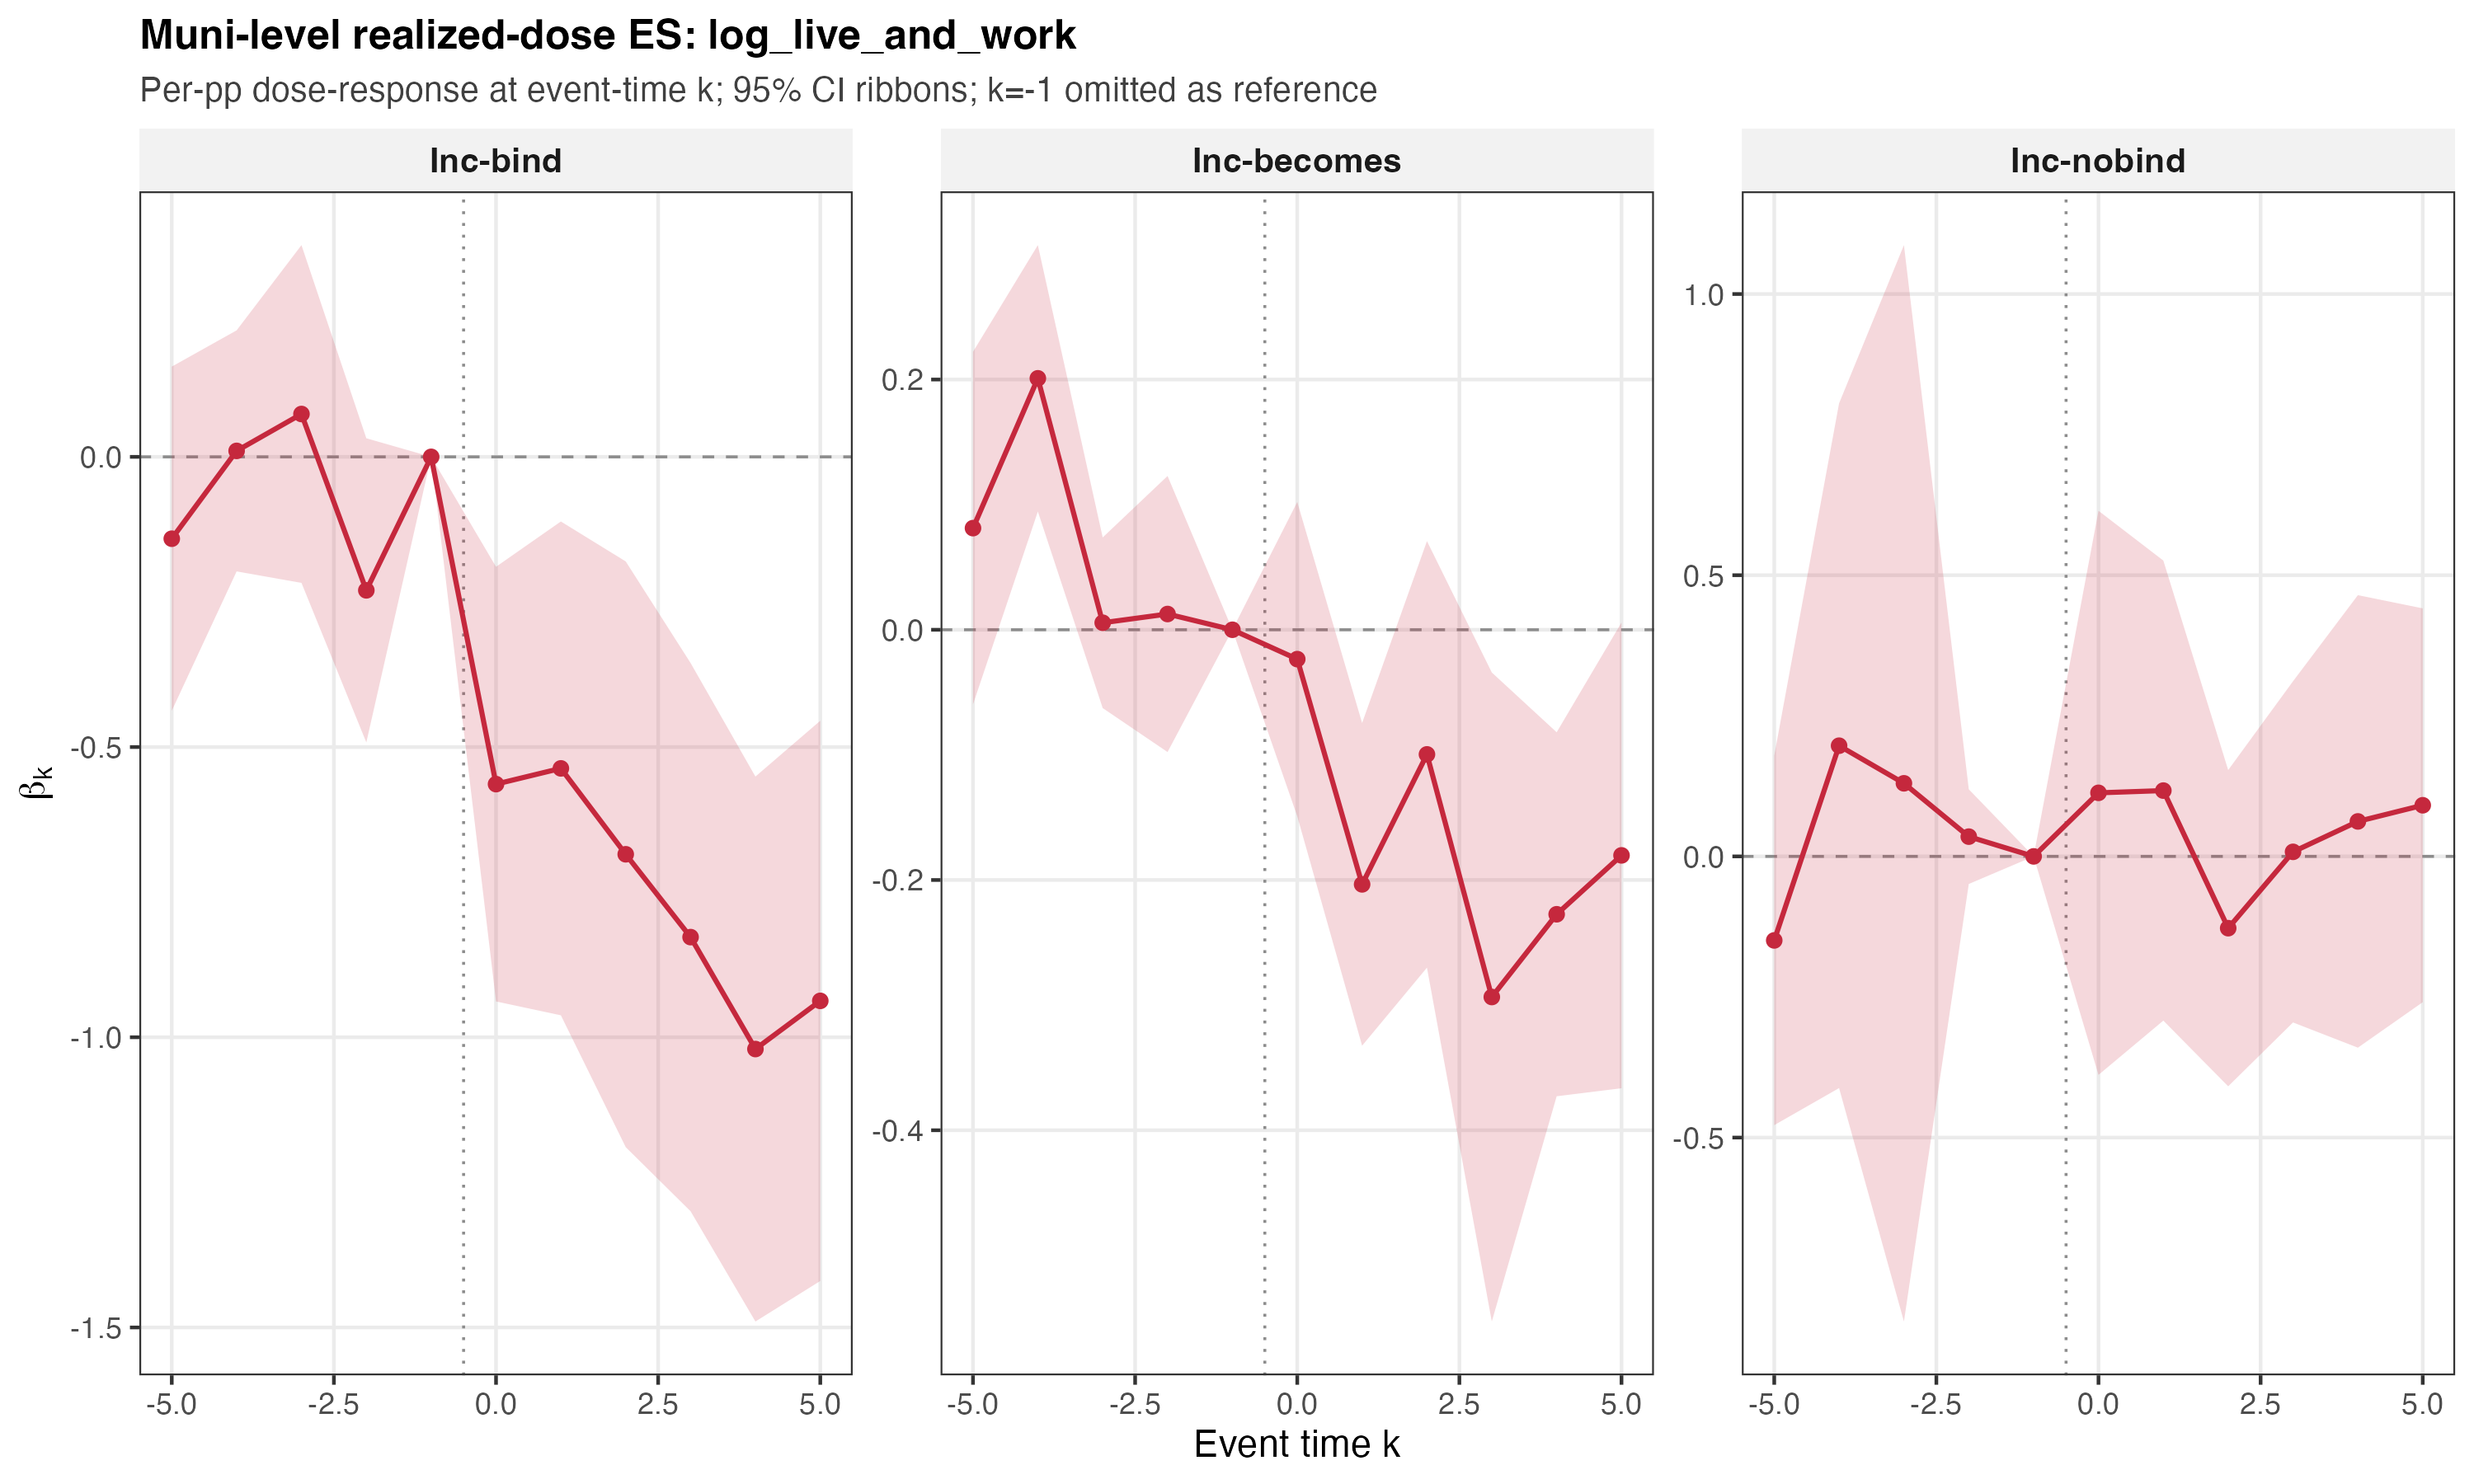
\includegraphics[width=0.95\textwidth]{../figures/es_realized_log_live_and_work.png}
  \begin{minipage}{0.95\textwidth}
    \footnotesize \textit{Notes:} Per-pp coefficient at each event-time, faceted by cell. Inc-bind pre-event Wald $p=0.33$; post path monotonically negative.
  \end{minipage}
\end{figure}

%==========================================================
\subsection{Summary}
\label{subsec:results-summary}

The headline finding is from the muni-level binding decomposition:
a 1 pp Inc-bind resident-rate increase reduces log live-and-work
by $-0.573^{***}$ with a clean realized-dose pre-trend
($p=0.33$) and a null Inc-nobind within-design placebo
($-0.082$, SE $0.143$). The same scaling on log in-commuters
gives $-0.421^{***}$. The pooled Inc benchmark in
Section~\ref{subsec:results-pooled} averages binding and
non-binding events, attenuating the Inc-bind effect to
$-0.232^{**}$; the decomposition recovers the binding-channel
response. Dec cells are dropped from the headline because they
fail pre-trends across the board and the cohort is thin. Full
coefficient tables with fiscal controls are in the appendix.

\section{Robustness}
\label{sec:robustness}
%==========================================================

This section summarizes the robustness checks behind the headline
muni-level dose-response. The realized-dose event-study pre-trend
diagnostic was discussed alongside the headline in
Section~\ref{subsubsec:decomp-es}. Full tables behind the
robustness summaries are in Appendix~\ref{app:robustness}.

\subsection{Pre/Post Act 32 Decomposition}
\label{subsec:rob-act32}

Splitting the headline cell-$\times$-dose specification at the Act-32
enforcement break (cohort first event year $<2012$ vs $\geq 2012$)
shows the municipality-level binding-cell effect strengthens after
consolidated employer withholding takes effect ($-0.593^{**}$ pre vs
$-0.546^{***}$ post on log residents working in own municipality)
(\hyperref[app:rob-act32]{see Appendix~\ref{app:rob-act32}}).

\subsection{Act 47 Distressed-Municipality Exclusion}
\label{subsec:rob-act47}

The Inc-bind cohort can include Act~47 distressed cities
\citep{paAct47_1987}, because Act~47 is the legal designation that
lets a municipality exceed the $0.5\%$ statutory municipality-EIT
cap. Selection-on-distress is therefore a candidate confounder: an
Act~47 designation typically follows a period of population
decline, so the rate hike happens after the municipality is
already losing residents and bundles with state oversight, debt
restructuring, and service cuts. After the flip-flopper drop,
$2$ of the $24$ Inc-bind municipalities match the DCED Act~47
designation list (Carbondale and Hazleton); the other historically
Act-47-designated PA cities (e.g.\ Braddock, Coatesville, Johnstown)
do not appear in the Inc-bind cell here because they have
non-monotone rate trajectories and were removed by the headline
sample filter (Section~\ref{subsec:stacked-continuous}).
Table~\ref{tab:act47_robustness} re-estimates the
municipality-level Inc-bind coefficient on the remaining $22$
non-Act-47 Inc-bind municipalities.

\begin{table}[H]
  \centering
  \caption{Act~47 robustness: dropping distressed Inc-bind municipalities from the cousub headline}
  \label{tab:act47_robustness}
  \small
  \begin{tabular}{lcc}
    \toprule
    Outcome & All 24 Inc-bind & Drop 2 Act~47 \\
    \midrule
    log live-and-work & $-0.718^{***}$ (0.214) & $-0.482^{**}$ (0.191) \\
    log in-commuters & $-0.540^{***}$ (0.165) & $-0.419^{**}$ (0.172) \\
    log total jobs & $-0.621^{***}$ (0.172) & $-0.462^{***}$ (0.167) \\
    live-in-muni share & $-0.059^{***}$ (0.020) & $-0.034^{**}$ (0.015) \\
    \bottomrule
  \end{tabular}
  \vspace{0.3em}
  \begin{minipage}{0.85\textwidth}
    \footnotesize \textit{Notes:} Muni-level Inc-bind coefficient on each residence-side outcome, with same FE / cluster / controls as the headline. Column 1 is the headline (all 24 Inc-bind municipalities). Column 2 drops 2 Act 47 distressed-designation municipalities from the Inc-bind cohort; the remaining 22 Inc-bind municipalities are mostly Home Rule and Boroughs. Cluster-robust SEs in parentheses. $^{*}p<0.10$, $^{**}p<0.05$, $^{***}p<0.01$.
  \end{minipage}
\end{table}



The point estimates are direction-preserving and modestly smaller
when the two Act~47 munis are dropped: the live-and-work
coefficient moves from $-0.71$ to $-0.47$, in-commuters from
$-0.53$ to $-0.41$, and share-live-in from $-0.060$ to $-0.034$.
All four coefficients remain statistically significant at $5\%$
or better on the trimmed sample, so the headline is not an artifact
of Act~47 selection. The attenuation when Act~47 cities are
removed is consistent with those two cities having larger realized
doses (each is on a steeper post-event rate path than the rest of
the Inc-bind cohort).

%==========================================================
\section{Discussion}
\label{sec:discussion}
%==========================================================

The continuous stacked DiD design produces a single headline
finding at the municipality level.

The central finding is that sorting is identified through the
binding channel. At the typical Inc-bind realized dose of
$0.24$ pp cumulative over five years, the muni resident-rate
increase reduces the log count of workers who both live and work in
the municipality by roughly $13\%$
($\beta = -0.573$ per pp, scaled to the typical event); the Inc-nobind
placebo---rate hikes whose post-event home stack remains below the
nonresident rate---is statistically indistinguishable from zero on
the same outcome ($-0.082$, $\text{SE} = 0.143$), and Inc-becomes
lies between the two. The pattern matches the institutional rule's
prediction: the same statutory rate change can produce a strong,
moderate, or null behavioral response depending solely on whether
the rate moves the worker's bill. This is direct evidence that
workers respond to taxes they actually pay rather than to statutory
rates per se. The per-pp coefficient ($-0.573$, or about $33\%$ per
pp) is the regression slope and should not be read as a
typical-event magnitude: a $1$ pp shock is two to three standard
deviations above the median realized dose in this cohort.

Identification at the municipality level is supported by the
realized-dose pre-trend diagnostic: the joint Wald test on
$k \leq -2$ leads of the Inc-bind cell does not reject parallel
trends ($p = 0.33$). The 24-municipality Inc-bind cohort (after
the flip-flopper drop) is therefore the defensible per-pp causal
quantity in this paper, but it is a small, eastern-PA-concentrated
set of Home Rule boroughs and Act~47 designees. The estimate is a
local treatment effect for binding rate-raisers, not a state-average
elasticity.

The in-commuters coefficient is also negative
($-0.412^{\ast\ast\ast}$), which is larger than a pure
within-commuting-zone residential-sorting story would predict. If
residents only relocated their home address while keeping their
job in the rate-raising muni, in-commuters would
\emph{rise}---someone has to fill the displaced residents' jobs.
I initially considered whether this in-commuter response reflects
joint resident- and nonresident-rate ordinances: if Inc-bind munis
were raising $\tau^M$ and $\tau^{\text{nr,M}}$ at the same time,
in-commuters would mechanically face a higher withholding bill on
their own paychecks and the negative coefficient would have a
direct work-side tax-bill explanation.
Table~\ref{tab:joint_event_diagnostic} rejects this hypothesis:
$20$ of $24$ Inc-bind munis change only the resident rate at the
first-event year, and the within-muni
$\Delta\tau^M$--$\Delta\tau^{\text{nr,M}}$ correlation is $+0.30$,
modest and the wrong sign for a mechanical work-side story (in
Inc-becomes and Inc-nobind cells the within-muni correlation is
actually negative). The negative in-commuters coefficient therefore
reflects a broader local labor-market response to muni fiscal
stress, consistent with workers and jobs both contracting when the
binding home-side rate rises rather than a mechanical taxation of
in-commuters' bills.

\begin{table}[!htbp]
  \centering
  \caption{Within-muni co-movement of resident-rate and nonresident-rate changes, by cell}
  \label{tab:joint_event_diagnostic}
  \footnotesize
  \renewcommand{\arraystretch}{1.0}
  \begin{tabular}{lrrrrr}
    \toprule
    Cell & Munis & First events & Joint $\Delta\tau^M{+}\Delta\tau^{\text{nr}}$ & $\tau^M$ only & $\Delta\tau^M$-$\Delta\tau^{\text{nr,M}}$ within-muni $r$ \\
    \midrule
    Inc-bind     & 24 & 24 & 4  & 20 & $+0.30$ \\
    Inc-becomes  & 39 & 39 & 0  & 39 & $-0.35$ \\
    Inc-nobind   & 14 & 14 & 5  & 9  & $-0.41$ \\
    \bottomrule
  \end{tabular}
  \vspace{0.3em}
  \begin{minipage}{0.95\textwidth}
    \footnotesize \textit{Notes:} The fourth and fifth columns count how each cell's first-event year decomposes: "Joint" rows have a non-zero $\Delta\tau^{\text{nr,M}}$ in the same year as the first $\Delta\tau^M$ event; "$\tau^M$ only" rows have $\Delta\tau^{\text{nr,M}} = 0$ in the event year. The sixth column reports the within-muni Pearson correlation between annual first differences $\Delta\tau^M_{i,t}$ and $\Delta\tau^{\text{nr,M}}_{i,t}$, restricted to muni-years with a non-zero change on at least one side. Inc-bind munis overwhelmingly raise $\tau^M$ without touching $\tau^{\text{nr,M}}$ in the same ordinance (20 of 24 first events).
  \end{minipage}
\end{table}


The joint regression also separates the two rate-setting channels,
and the muni-versus-SD sign contrast is itself a finding rather
than something to explain away. The muni resident-rate Inc-bind
coefficient is large and negative, while the SD resident-rate
coefficient in the same joint regression is small and
\emph{positive} ($+0.177^{\ast}$ on the live-and-work outcome).
This contrast is what a tax-amenity-bundle model predicts: SD
revenues primarily fund school quality, which capitalizes into the
willingness to pay to reside in the district
\citep{blackBetterSchoolsTaxes1999, bayerFerreiraMcMillan2007},
while muni-resident-rate revenue funds streets, debt service,
intergovernmental transfers, and general administration---less
salient amenities that differentiate municipalities much less
across PA's small cousubs. Workers respond to the bundle of (taxes
$\times$ amenities) rather than to statutory rates generically.
The sign contrast is direct evidence of bundle-level Tiebout
sorting and strengthens the binding-channel interpretation rather
than complicating it: the binding rule tells us \emph{which} rate
events move workers' bills, and the rate-setter contrast tells us
\emph{how} workers value the revenue once collected.

The treated cohort can also include Act~47 distressed cities, which
raises a selection-on-distress concern: Act~47 designation
typically follows a period of decline and bundles rate-hike
authority with state oversight, debt restructuring, and service
cuts. Section~\ref{subsec:rob-act47} re-estimates the headline
excluding the $2$ Act~47 Inc-bind municipalities (Carbondale and
Hazleton) out of the $24$-municipality Inc-bind cohort
(Table~\ref{tab:act47_robustness}); the point estimates are
direction-preserving and modestly smaller (live-and-work moves from
$-0.71$ to $-0.47$, share-live-in from $-0.060$ to $-0.034$),
with all four coefficients remaining statistically significant at
$5\%$ or better on the trimmed sample. The binding mechanism is
therefore not a relabelling of Act~47 fiscal distress.

Six limitations merit acknowledgment. First, the LODES OD data
covers PA municipalities but not cross-state inflows in the
intra-state main file used here; the auxiliary file (cross-state
inflows) is downloaded but not yet incorporated, which would
tighten the estimates of in-commuters for border municipalities.

Second, the paper estimates the residential-sorting response to the
home-side resident rate but does not separately estimate the
work-side response to the municipality nonresident rate ($\tau^{\text{nr}}$).
The nonresident rate enters the design only through the
binding classification of cells. A complementary work-side
specification---estimating in-commuter and total-jobs responses to
$\tau^{\text{nr}}$ events at the municipality level, with a parallel
binding decomposition---would test the workplace-side
response separately. I defer this to a separate paper.

Third, the per-pp coefficient is a displacement elasticity, not a
net-out-of-Pennsylvania-sorting elasticity, and this distinction
matters more in PA than in most settings because municipalities are
small and dense. The Inc-bind cohort is concentrated in eastern PA
(Figure~\ref{fig:pa_map}); a worker leaving Hazleton for an
adjacent muni shows up as a $-1$ in the Hazleton live-and-work
count and a $+1$ to that neighbor's residence count---a within-CZ
relocation, not an exit from PA's labor market or tax base. The
headline specification partially absorbs neighbor-rate variation
through never-changed-only controls and municipality-by-stack
fixed effects, but it does not formally model spatial spillovers,
and a worker moving to an adjacent muni whose rate is also moving
violates SUTVA. The $-0.573$ coefficient should therefore be
interpreted as the marginal effect of a rate hike on the
\emph{geographic distribution} of workers within commuting
distance, not on the size of PA's economy or PA's residential tax
base. The
\citet{buttsDifferenceinDifferencesEstimationSpatial2023}
estimator generalizes stacked DiD to allow for SUTVA violations
from spatial spillovers across treated units, using an explicit
spatial weighting matrix on the adjacency graph. Applying it to
the PA municipality adjacency graph is left for future work and is
the natural next step for separating displacement from
out-of-state sorting in this setting.

Fourth, I do not currently estimate the headline using the
heterogeneity-robust continuous-treatment difference-in-differences
estimator of \citet{dechaisemartinDifferenceinDifferencesEstimatorsTreatments2022}, which generalizes
the de~Chaisemartin--D'Haultf{\oe}uille framework
\citep{dechaisemartinTwoWayFixedEffects2020, dechaisemartinTwoWayFixedEffects2023} to
continuously distributed treatments at every period and leverages
switchers (units that move both up and down in dose) for
identification. A municipality-level CDH cross-check would provide an
additional robustness benchmark for the Inc-bind coefficient, but the
package documentation and switcher-based identification at the
dose scale present in this panel are not yet stable, and the
cross-check is left for future work
\citep{chaisemartinUsingDid_multiplegt_dynEstimate2025}.

Fifth, LODES is a stock dataset rather than a person-linked
flow dataset. For each (residence muni, workplace muni, year), I
observe a count of workers; I do not observe individual migration
histories. The headline coefficient on the muni count of residents
is therefore a net elasticity---the combined effect of move-outs
and move-ins---rather than separate estimates of the gross outflow
and gross inflow margins. The paper's evidence that municipal rate
hikes reduce the residential count is consistent both with workers
leaving and with workers not arriving to replace those who left;
LODES alone cannot decompose the two. Decomposing into gross
outflow and gross inflow would require person-linked
administrative data: the IRS Statistics of Income individual master
file, the American Community Survey microdata with full
residence-history linkage, or---most directly---the LEHD
Job-to-Job Flows file, which tracks the same workers across
employer transitions at quarterly frequency. All three are
restricted-access products requiring approved-project status under
the Census Bureau's Federal Statistical Research Data Centers
(FSRDCs) or IRS Statistics of Income agreements; the microdata
cannot be exported and must be analyzed at a physical FSRDC
location. Replicating the present analysis on person-linked data
is a clear extension but a substantially larger undertaking with
its own access timeline.

Sixth, the paper does not estimate a comparable elasticity for
the property tax, the other major local-revenue lever in
Pennsylvania. The Oates (1969) capitalization theory predicts a
substantially smaller residential-sorting elasticity for property
tax than for the EIT, because property tax falls on owners and
capitalizes into house prices rather than on workers directly.
Estimating a comparable property-tax elasticity would test the
falsification implication ``is the EIT effect specifically about the
EIT, or any local tax raising?'' but requires a 2002--2019 municipality-level
millage panel that DCED does not publish (the DCED Annual Financial Report schema dropped per-municipality
millage in 2006). Constructing this panel from county assessor
records is left for future work.

%==========================================================
\section{Conclusion}
\label{sec:conclusion}
%==========================================================

When do local income taxes cause residential sorting? In
Pennsylvania, when the piecewise max-rule makes the statutory rate
increase change the worker's actual bill. At the typical Inc-bind
realized dose of $0.24$ pp cumulative over five years, the muni
resident-rate increase reduces the count of workers who both live
and work in their own municipality by roughly $13\%$
($\beta = -0.573$ per pp, scaled by the typical event), with clean
realized-dose pre-trends (joint Wald $p = 0.33$) and a null
Inc-nobind within-design placebo ($-0.082$, $\text{SE} = 0.143$)
on the same outcome. The response is therefore tied to tax
liability rather than to the statutory rate change itself, and the
binding decomposition is what distinguishes the two. The per-pp
coefficient ($-0.573$, or roughly $33\%$ per pp) is the regression
slope, not a typical-event headline; the estimate is identified on
a small, eastern-PA cohort of binding rate-raisers, so it is a
local treatment effect rather than a state-average elasticity.

The methodological contribution is to deliver within-design
heterogeneity of the kind that
\citet{agrawalLessonsStateLocal} identifies as missing from the
US local-income-tax literature: the piecewise EIT rule splits
otherwise-identical statutory rate increases into a treated cell
that moves the worker's bill (Inc-bind) and a within-design
placebo cell that does not (Inc-nobind), making the design
self-falsifying in a way that pooled local-tax regressions are not.
The complementary muni-versus-SD sign contrast---negative on the
muni rate, positive on the SD rate in the same joint regression---is
consistent with bundle-level Tiebout sorting: workers respond to
the (taxes $\times$ amenities) bundle, and SD revenues fund the
amenity (school quality) that capitalizes into willingness to
reside in the district.

The natural next step is a companion paper on the
work-side response to the muni nonresident rate, $\tau^{\text{nr}}$,
which enters the present design only through the binding
classification of cells. Together the two papers would cover both
sides of the piecewise max-rule.

The same design framework---a continuous stacked DiD with binding
decomposition, a realized-dose event study as a
strong-parallel-trends diagnostic, and a within-design placebo
cell whose theoretical prediction is zero---is portable to other
settings where a piecewise tax rule generates predictable
cross-sectional variation in whether a statutory rate change moves
the worker's bill. Local sales taxes with use-tax-credit rules,
county-level income-tax credits across state borders, and special
tax districts with overlapping jurisdictions are candidate
extensions.

% \section*{Acknowledgments}
% TODO: fill in before submission

%==========================================================
% BIBLIOGRAPHY
%==========================================================
\printbibliography

%==========================================================
% APPENDIX
%==========================================================
\appendix

%==========================================================
\section{Full Results with Control Coefficients}
\label{app:full-results}
%==========================================================

This appendix reports the muni-level binding-decomposition
regression with the fiscal-control coefficients and diagnostics.
Table~\ref{tab:app_full_muni_cell_results} reports the muni-rate
cells with controls and Table~\ref{tab:app_full_muni_sd_side_results}
reports the SD-rate cells from the same joint regression.

\begin{table}[!htbp]
  \centering
  \caption{Municipality-level dose-response: muni resident-rate cells with fiscal controls (full spec)}
  \label{tab:app_full_muni_cell_results}
  \footnotesize
  \renewcommand{\arraystretch}{0.9}
  \resizebox{\textwidth}{!}{
  \begin{tabular}{lcccc}
    \toprule
    Outcome & Log(work in own muni) & Log(in-commuters) & Log(employed residents) & Share live in muni \\
    \midrule
    \textbf{Inc-bind} & -0.573\sym{***} & -0.421\sym{***} & -0.104\sym{**} & -0.057\sym{***} \\
                      & (0.162) & (0.126) & (0.043) & (0.020) \\
    \textbf{Inc-becomes} & -0.239\sym{***} & -0.247\sym{***} & -0.040 & -0.012 \\
                      & (0.055) & (0.055) & (0.026) & (0.011) \\
    \textbf{Inc-nobind} & -0.082 & -0.657 & 0.235\sym{***} & -0.015 \\
                      & (0.143) & (0.653) & (0.077) & (0.027) \\
    \textbf{Dec-bind} & 0.222\sym{*} & 0.152 & 0.077 & 0.010\sym{***} \\
                      & (0.114) & (0.107) & (0.138) & (0.002) \\
    \textbf{Dec-becomes-non} & -1.221\sym{***} & 0.184\sym{**} & -1.482\sym{***} & -0.146\sym{***} \\
                      & (0.071) & (0.072) & (0.033) & (0.005) \\
    \textbf{Dec-nobind} & --- & 0.150\sym{***} & -0.228\sym{***} & 0.013\sym{***} \\
                      &  & (0.010) & (0.005) & (0.001) \\
    \midrule
    \multicolumn{5}{l}{\textit{Fiscal controls}} \\
    police-services share & 0.104 & -0.015 & 0.005 & 0.008 \\
                      & (0.100) & (0.104) & (0.058) & (0.007) \\
    streets share & 0.051 & 0.006 & -0.001 & 0.002 \\
                      & (0.040) & (0.040) & (0.019) & (0.003) \\
    debt-service share & -0.052 & -0.021 & 0.018 & 0.004 \\
                      & (0.051) & (0.058) & (0.029) & (0.005) \\
    EIT-revenue share & -0.024 & 0.261\sym{***} & 0.017 & -0.013\sym{*} \\
                      & (0.086) & (0.084) & (0.041) & (0.007) \\
    real-estate-tax share & -0.180\sym{**} & -0.263\sym{***} & -0.040 & -0.008 \\
                      & (0.087) & (0.094) & (0.041) & (0.007) \\
    intergovernmental-revenue share & 0.027 & 0.036 & 0.067\sym{***} & 0.005 \\
                      & (0.044) & (0.048) & (0.023) & (0.004) \\
    \midrule
    $N$ & 193,699 & 211,780 & 215,159 & 211,789 \\
    $R^2$ & 0.964 & 0.960 & 0.981 & 0.825 \\
    Within $R^2$ & 0.001 & 0.001 & 0.001 & 0.001 \\
    Dep.\ mean & 3.663 & 5.839 & 6.688 & 0.093 \\
    Dep.\ SD & 1.920 & 1.878 & 1.294 & 0.075 \\
    \bottomrule
  \end{tabular}
  }
  \vspace{0.3em}
  \begin{minipage}{0.95\textwidth}
    \footnotesize \textit{Notes:} Stacked-DiD; muni$\times$stack and year$\times$stack FE; SE clustered at muni. SE in parens. $^{*}p<0.10$, $^{**}p<0.05$, $^{***}p<0.01$.
  \end{minipage}
\end{table}


\begin{table}[!htbp]
  \centering
  \caption{Municipality-level dose-response: SD resident-rate cells with fiscal controls (full spec)}
  \label{tab:app_full_muni_sd_side_results}
  \footnotesize
  \renewcommand{\arraystretch}{0.9}
  \resizebox{\textwidth}{!}{
  \begin{tabular}{lcccc}
    \toprule
    Outcome & Log(work in own muni) & Log(in-commuters) & Log(employed residents) & Share live in muni \\
    \midrule
    \textbf{Inc-bind} & 0.165 & 0.159 & 0.057 & 0.005 \\
                      & (0.109) & (0.096) & (0.049) & (0.007) \\
    \textbf{Inc-becomes} & 0.084 & 0.086 & 0.031 & 0.007 \\
                      & (0.095) & (0.089) & (0.056) & (0.007) \\
    \midrule
    \multicolumn{5}{l}{\textit{Fiscal controls}} \\
    police-services share & 0.111 & -0.041 & -0.001 & 0.009 \\
                      & (0.104) & (0.107) & (0.058) & (0.007) \\
    streets share & 0.050 & 0.011 & 0.001 & 0.002 \\
                      & (0.041) & (0.041) & (0.019) & (0.003) \\
    debt-service share & -0.065 & -0.029 & 0.018 & 0.004 \\
                      & (0.054) & (0.060) & (0.030) & (0.005) \\
    EIT-revenue share & -0.036 & 0.236\sym{***} & 0.017 & -0.013\sym{*} \\
                      & (0.088) & (0.083) & (0.042) & (0.007) \\
    real-estate-tax share & -0.189\sym{**} & -0.274\sym{***} & -0.042 & -0.007 \\
                      & (0.090) & (0.096) & (0.043) & (0.007) \\
    intergovernmental-revenue share & 0.018 & 0.033 & 0.075\sym{***} & 0.005 \\
                      & (0.046) & (0.050) & (0.024) & (0.004) \\
    \midrule
    $N$ & 174,929 & 191,405 & 194,533 & 191,413 \\
    $R^2$ & 0.963 & 0.959 & 0.980 & 0.825 \\
    Within $R^2$ & 0.001 & 0.001 & 0.001 & 0.001 \\
    Dep.\ mean & 3.659 & 5.836 & 6.686 & 0.092 \\
    Dep.\ SD & 1.926 & 1.883 & 1.296 & 0.075 \\
    \bottomrule
  \end{tabular}
  }
  \vspace{0.3em}
  \begin{minipage}{0.95\textwidth}
    \footnotesize \textit{Notes:} Stacked-DiD; muni$\times$stack and year$\times$stack FE; SE clustered at muni. SD-side cell$\times$dose coefficients from the same regression as the muni-side full-spec table. Rows omitted (no estimable coefficients): Inc-nobind. SE in parens. $^{*}p<0.10$, $^{**}p<0.05$, $^{***}p<0.01$.
  \end{minipage}
\end{table}


%==========================================================
\section{Realized-Dose Event Studies, Full Set}
\label{app:es-realized}
%==========================================================

Per-cell realized-dose Sun--Abraham event studies at the muni
level for the remaining residence-side outcomes (log live-and-work
is in the body, \S\ref{subsubsec:decomp-es}).

\begin{figure}[H]
  \centering
  \caption{Muni-level realized-dose ES on $\log(\text{in-commuters})$, by cell.}
  \label{fig:app_es_realized_muni_incomm}
  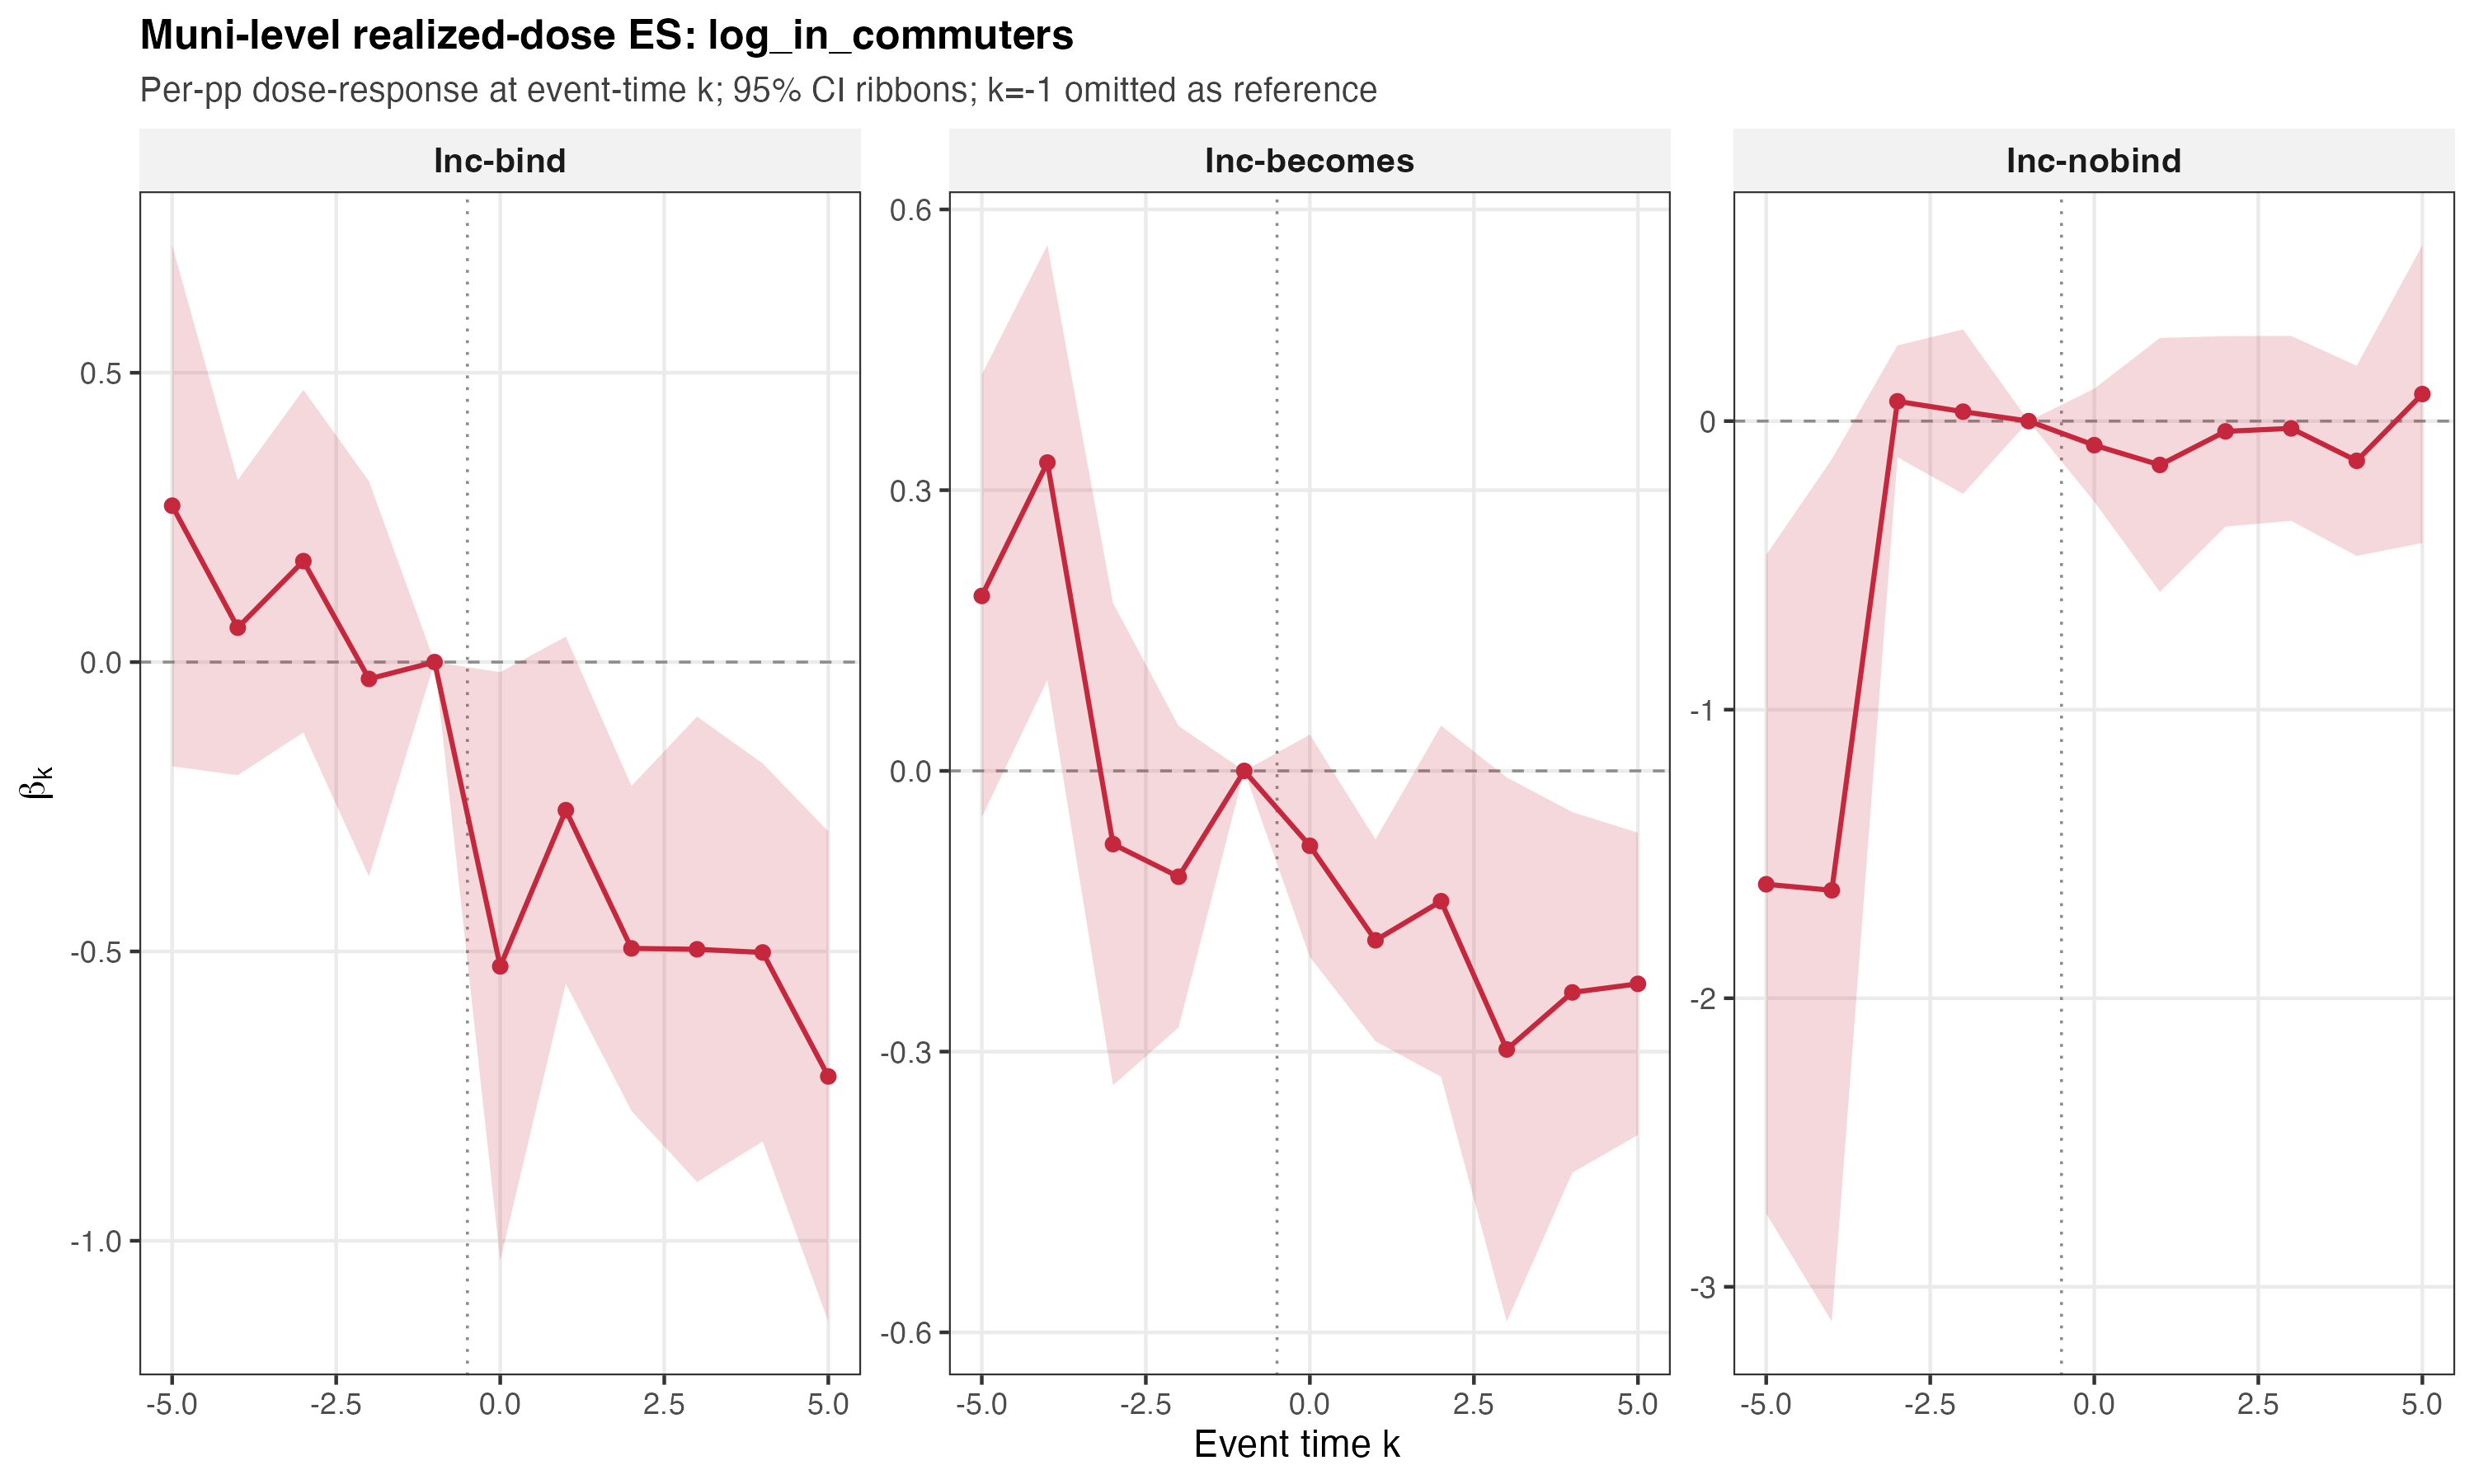
\includegraphics[width=0.95\textwidth]{../figures/es_realized_log_in_commuters.png}
\end{figure}

\begin{figure}[H]
  \centering
  \caption{Muni-level realized-dose ES on $\log(\text{total residents})$, by cell.}
  \label{fig:app_es_realized_muni_residents}
  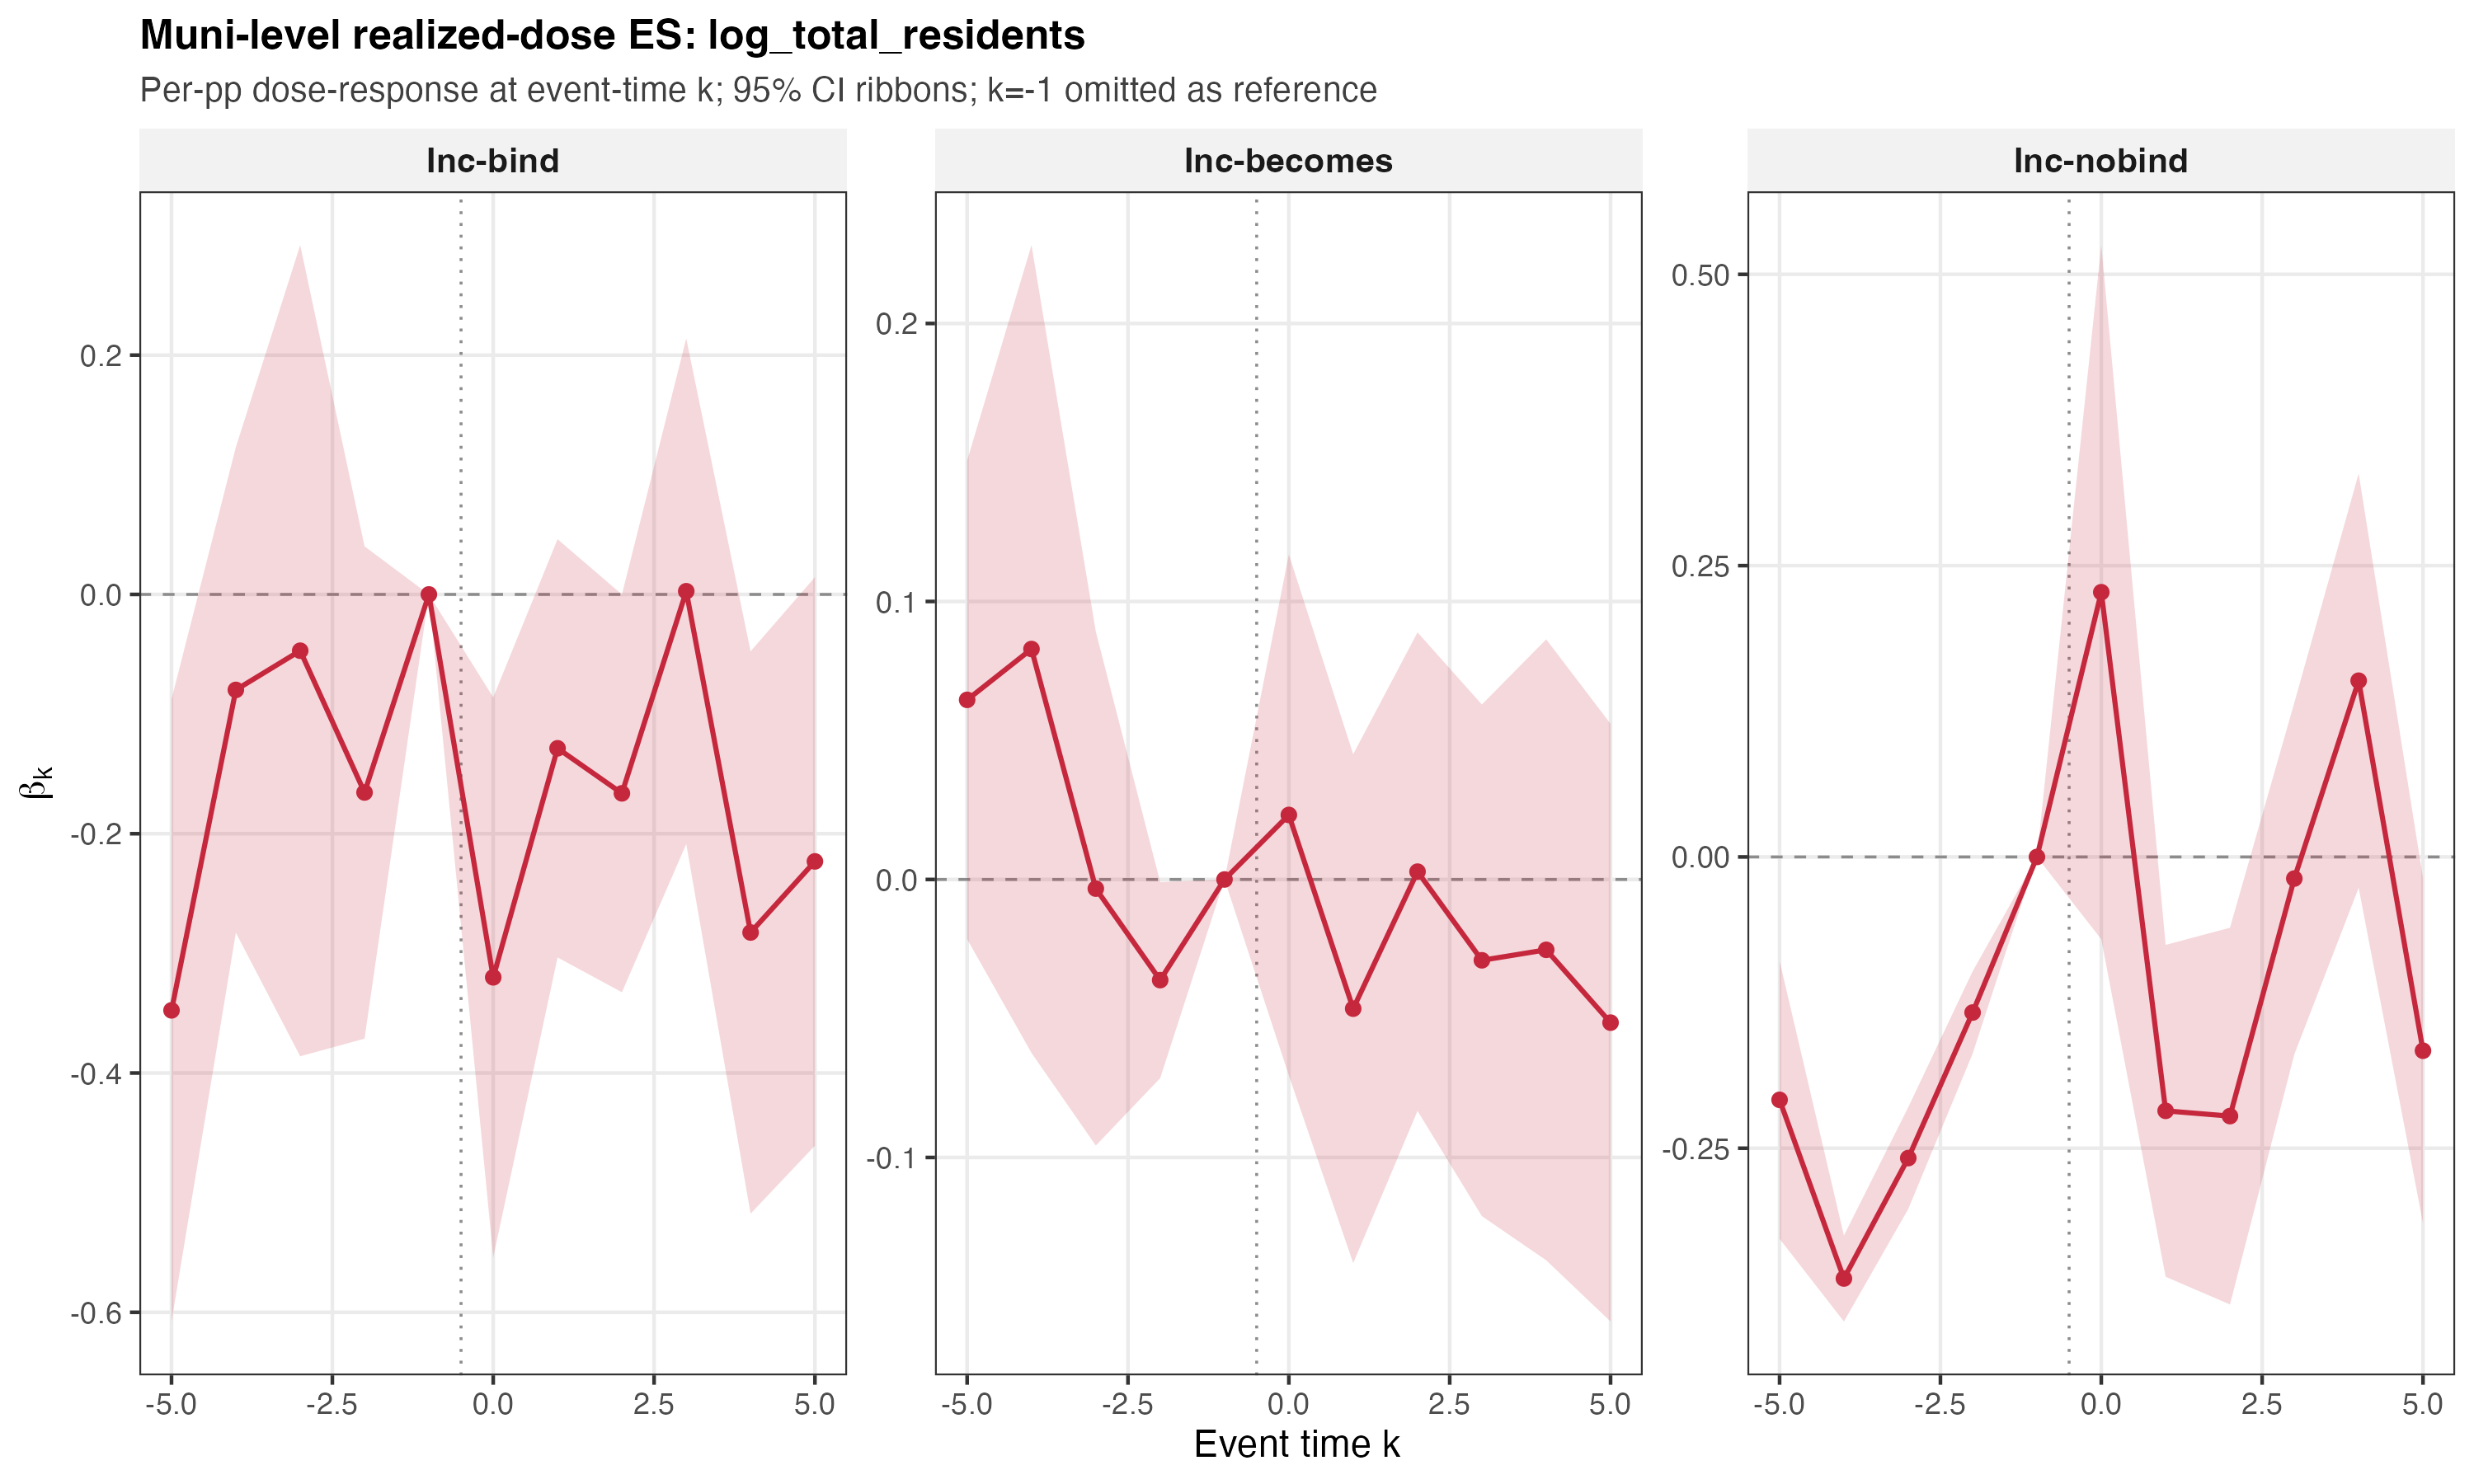
\includegraphics[width=0.95\textwidth]{../figures/es_realized_log_total_residents.png}
\end{figure}

\begin{figure}[H]
  \centering
  \caption{Muni-level realized-dose ES on the share of workers
           living in their own municipality, by cell.}
  \label{fig:app_es_realized_muni_share_in}
  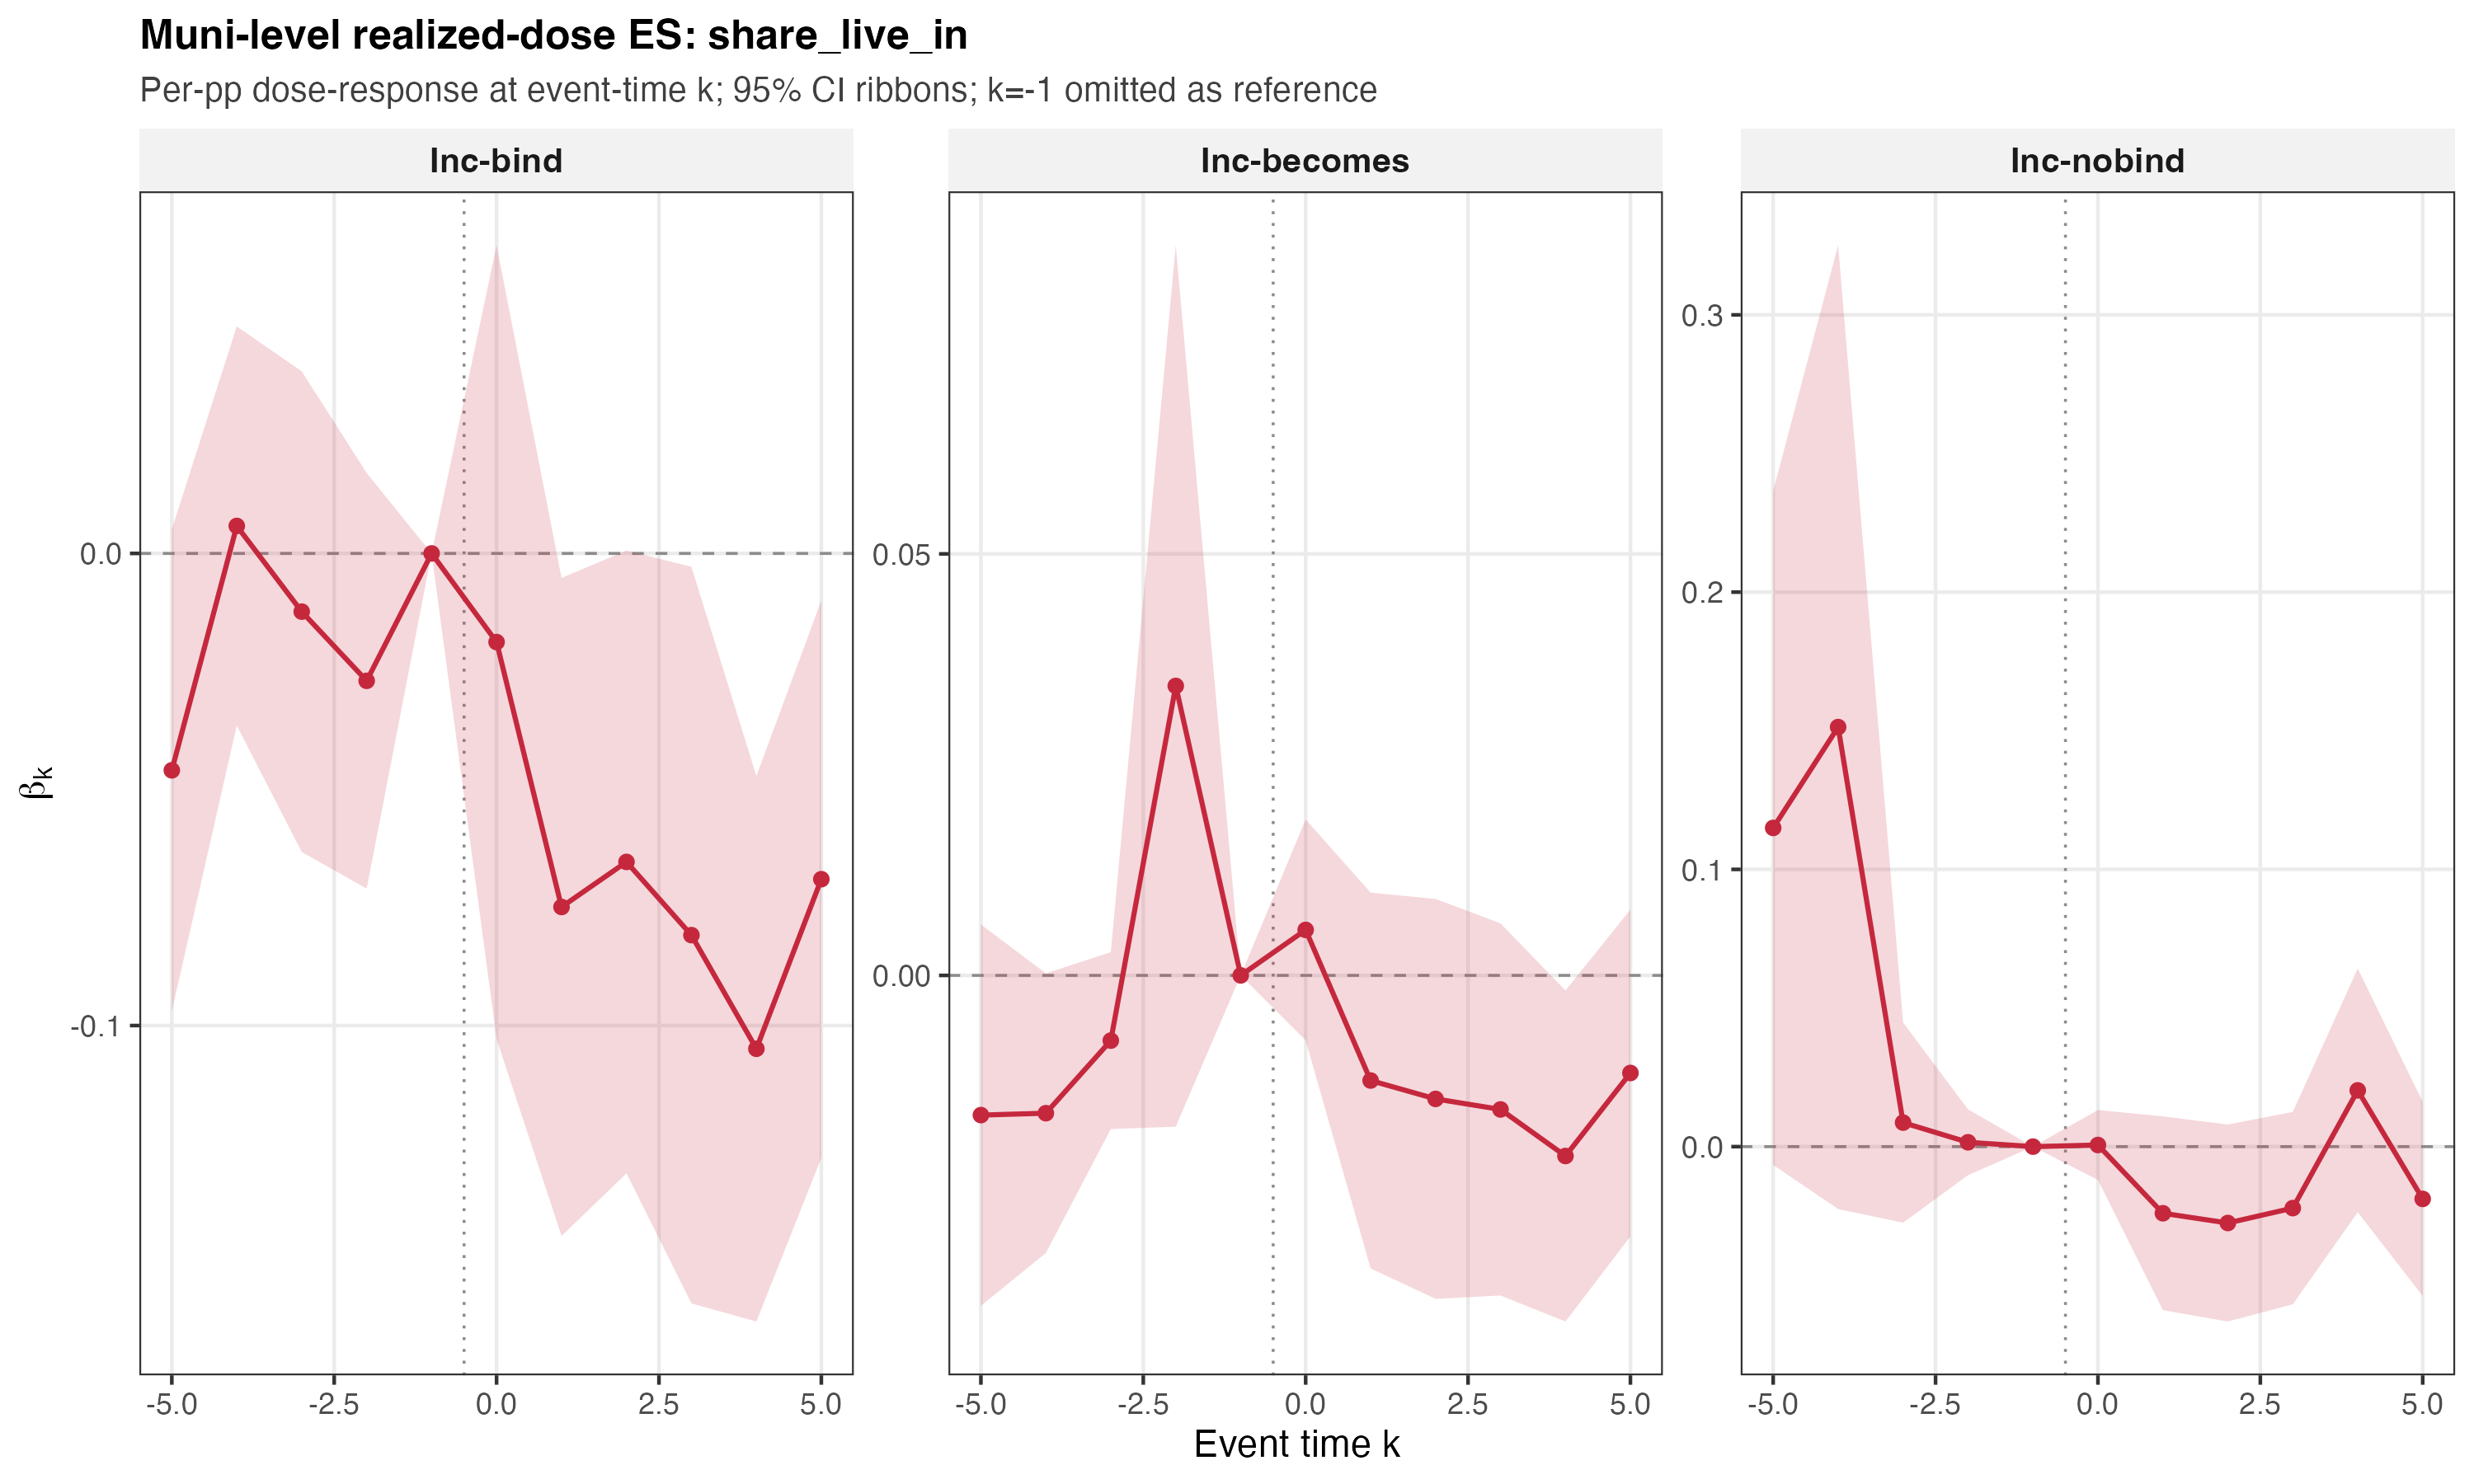
\includegraphics[width=0.95\textwidth]{../figures/es_realized_share_live_in.png}
\end{figure}

%==========================================================
\section{Robustness}
\label{app:robustness}
%==========================================================

Full tables behind the robustness summaries in
Section~\ref{sec:robustness}.

\subsection{Pre/post Act 32 split}
\label{app:rob-act32}

Headline cell $\times$ dose specification re-estimated on pre-Act-32
($c<2012$) and post-Act-32 ($c\geq 2012$) cohort subsamples at the
municipality level.

\begin{table}[H]
  \centering
  \caption{Pre-/post-Act-32 split --- municipality level}
  \label{tab:act32_cousub}
  \small
  \resizebox{\textwidth}{!}{
  \begin{tabular}{lcccc}
    \toprule
    Outcome & Log(work in own muni) & Log(in-commuters) & Log(employed residents) & Share live in muni \\
    \midrule
    \textbf{Inc-bind} & & & & \\
    \quad Pre-Act 32 & -0.339\sym{**} & -0.156 & -0.098\sym{**} & -0.047\sym{***} \\
                    & (0.138) & (0.112) & (0.045) & (0.013) \\
    \quad Post-Act 32 & -0.534\sym{***} & -0.334\sym{***} & -0.104\sym{***} & -0.040\sym{***} \\
                    & (0.075) & (0.080) & (0.034) & (0.004) \\
    \textbf{Inc-becomes} & & & & \\
    \quad Pre-Act 32 & -0.230\sym{**} & -0.239\sym{***} & -0.131\sym{*} & -0.029\sym{*} \\
                    & (0.093) & (0.089) & (0.074) & (0.016) \\
    \quad Post-Act 32 & -0.143 & -0.160 & -0.013 & 0.003 \\
                    & (0.106) & (0.108) & (0.019) & (0.009) \\
    \textbf{Inc-nobind} & & & & \\
    \quad Pre-Act 32 & -0.051 & -0.078 & -0.052\sym{**} & -0.013 \\
                    & (0.220) & (0.157) & (0.026) & (0.010) \\
    \quad Post-Act 32 & -0.094 & -0.305 & 0.365\sym{***} & -0.010 \\
                    & (0.113) & (0.368) & (0.095) & (0.013) \\
    \textbf{Dec-bind} & & & & \\
    \quad Pre-Act 32 & 0.341\sym{***} & 0.049 & -0.013 & 0.074\sym{*} \\
                    & (0.046) & (0.135) & (0.277) & (0.044) \\
    \quad Post-Act 32 & 0.068 & 0.056 & -0.133 & 0.008\sym{***} \\
                    & (0.144) & (0.183) & (0.102) & (0.003) \\
    \textbf{Dec-becomes-non} & & & & \\
    \quad Pre-Act 32 & -1.220\sym{***} & 0.177\sym{**} & -1.474\sym{***} & -0.144\sym{***} \\
                    & (0.069) & (0.071) & (0.032) & (0.005) \\
    \quad Post-Act 32 & 1.384\sym{***} & 0.874\sym{***} & 0.734\sym{***} & 0.057\sym{***} \\
                    & (0.106) & (0.112) & (0.053) & (0.008) \\
    \textbf{Dec-nobind} & & & & \\
    \quad Pre-Act 32 & 0.377\sym{***} & -0.211 & 0.397\sym{***} & 0.019 \\
                    & (0.106) & (0.218) & (0.018) & (0.047) \\
    \quad Post-Act 32 & 0.094\sym{***} & 0.177\sym{***} & -0.132 & 0.006 \\
                    & (0.019) & (0.027) & (0.090) & (0.006) \\
    \midrule
    \textit{Pre-Act 32} & & & & \\
    \quad $N$ & 218,438 & 238,760 & 242,447 & 238,770 \\
    \quad $R^2$ & 0.964 & 0.959 & 0.981 & 0.823 \\
    \quad Within $R^2$ & 0.001 & 0.001 & 0.001 & 0.001 \\
    \quad Dep.\ mean & 3.675 & 5.845 & 6.696 & 0.093 \\
    \quad Dep.\ SD & 1.933 & 1.886 & 1.298 & 0.075 \\
    \textit{Post-Act 32} & & & & \\
    \quad $N$ & 218,036 & 238,336 & 242,033 & 238,346 \\
    \quad $R^2$ & 0.964 & 0.959 & 0.981 & 0.823 \\
    \quad Within $R^2$ & 0.001 & 0.001 & 0.001 & 0.001 \\
    \quad Dep.\ mean & 3.672 & 5.843 & 6.695 & 0.093 \\
    \quad Dep.\ SD & 1.932 & 1.885 & 1.297 & 0.075 \\
    \bottomrule
  \end{tabular}
  }
  \vspace{0.3em}
  \begin{minipage}{0.95\textwidth}
    \footnotesize \textit{Notes:} Cluster-robust standard errors in parentheses. Treated cohorts split at first event year $c < 2012$ (Pre-Act~32) vs $c \geq 2012$ (Post-Act~32). At the muni level, the Inc-bind coefficient on log live-and-work strengthens from $-0.339^{**}$ (pre) to $-0.534^{***}$ (post), consistent with consolidated employer withholding making the EIT binding \citep{bagchiEffectsIntroducingWithholding2022}; the within-design placebo (Inc-nobind) is null in both periods. $^{*}p<0.10$, $^{**}p<0.05$, $^{***}p<0.01$.
  \end{minipage}
\end{table}


\subsection{Sample variants}
\label{app:rob-sample}

Three sample variants for the DCED nonresident-rate panel (strict,
filled, drop-incomplete) leave the headline municipality Inc-bind coefficient
on log live-and-work essentially unchanged at $-0.573^{***}$.

%==========================================================
\end{document}
